\documentclass[oneside]{book}\usepackage[]{graphicx}\usepackage[svgnames]{xcolor}
% maxwidth is the original width if it is less than linewidth
% otherwise use linewidth (to make sure the graphics do not exceed the margin)
\makeatletter
\def\maxwidth{ %
  \ifdim\Gin@nat@width>\linewidth
    \linewidth
  \else
    \Gin@nat@width
  \fi
}
\makeatother

\definecolor{fgcolor}{rgb}{0.345, 0.345, 0.345}
\newcommand{\hlnum}[1]{\textcolor[rgb]{0.686,0.059,0.569}{#1}}%
\newcommand{\hlstr}[1]{\textcolor[rgb]{0.192,0.494,0.8}{#1}}%
\newcommand{\hlcom}[1]{\textcolor[rgb]{0.678,0.584,0.686}{\textit{#1}}}%
\newcommand{\hlopt}[1]{\textcolor[rgb]{0,0,0}{#1}}%
\newcommand{\hlstd}[1]{\textcolor[rgb]{0.345,0.345,0.345}{#1}}%
\newcommand{\hlkwa}[1]{\textcolor[rgb]{0.161,0.373,0.58}{\textbf{#1}}}%
\newcommand{\hlkwb}[1]{\textcolor[rgb]{0.69,0.353,0.396}{#1}}%
\newcommand{\hlkwc}[1]{\textcolor[rgb]{0.333,0.667,0.333}{#1}}%
\newcommand{\hlkwd}[1]{\textcolor[rgb]{0.737,0.353,0.396}{\textbf{#1}}}%
\let\hlipl\hlkwb

\usepackage{framed}
\makeatletter
\newenvironment{kframe}{%
 \def\at@end@of@kframe{}%
 \ifinner\ifhmode%
  \def\at@end@of@kframe{\end{minipage}}%
  \begin{minipage}{\columnwidth}%
 \fi\fi%
 \def\FrameCommand##1{\hskip\@totalleftmargin \hskip-\fboxsep
 \colorbox{shadecolor}{##1}\hskip-\fboxsep
     % There is no \\@totalrightmargin, so:
     \hskip-\linewidth \hskip-\@totalleftmargin \hskip\columnwidth}%
 \MakeFramed {\advance\hsize-\width
   \@totalleftmargin\z@ \linewidth\hsize
   \@setminipage}}%
 {\par\unskip\endMakeFramed%
 \at@end@of@kframe}
\makeatother

\definecolor{shadecolor}{rgb}{.97, .97, .97}
\definecolor{messagecolor}{rgb}{0, 0, 0}
\definecolor{warningcolor}{rgb}{1, 0, 1}
\definecolor{errorcolor}{rgb}{1, 0, 0}
\newenvironment{knitrout}{}{} % an empty environment to be redefined in TeX

\usepackage{alltt}
\usepackage[svgnames]{xcolor}
\usepackage[british]{babel}
\usepackage[protrusion,expansion,babel,final]{microtype}
\usepackage[margin=1in]{geometry}
\usepackage[pdfversion=1.7]{hyperref}
\usepackage[shortlabels]{enumitem}
\usepackage{graphicx}
\usepackage{mathtools}
\usepackage{cleveref}
\usepackage{booktabs}
\usepackage{nicematrix}
\usepackage{derivative}
\usepackage{etoolbox}
\usepackage{siunitx}
\usepackage{lmodern}
\usepackage[T1]{fontenc}
\usepackage[scaled=.98]{XCharter}
\usepackage[scaled=1.04,varqu,varl]{inconsolata}% inconsolata typewriter
\usepackage{amssymb}
\makeatletter
\@namedef{T1/zi4/m/it}{<->ssub*lmr/m/it}
\makeatother

\usepackage{bm}
\usepackage{tikz}
\usepackage{float}

% Functions
\providecommand\given{} % just to make sure it exists
\DeclarePairedDelimiterXPP{\E}[1]{\operatorname{\mathbb{E}}}[]{}{%
    \renewcommand\given{\nonscript\:\delimsize\vert\nonscript\:\mathopen{}}%
    \ifblank{#1}{\:\cdot\:}%
    #1}%
\DeclarePairedDelimiterXPP{\estE}[1]{\operatorname{\widehat{\mathbb{E}}}}[]{}{%
    \renewcommand\given{\nonscript\:\delimsize\vert\nonscript\:\mathopen{}}%
    \ifblank{#1}{\:\cdot\:}%
    #1}%
\DeclarePairedDelimiterXPP{\V}[1]{\operatorname{\textsf{V}}}(){}{%
    \renewcommand\given{\nonscript\:\delimsize\vert\nonscript\:\mathopen{}}%
    \ifblank{#1}{\:\cdot\:}%
    #1}%
\DeclarePairedDelimiterXPP{\Var}[1]{\operatorname{\textsf{Var}}}(){}{%
    \renewcommand\given{\nonscript\:\delimsize\vert\nonscript\:\mathopen{}}%
    \ifblank{#1}{\:\cdot\:}%
    #1}%
\DeclarePairedDelimiterXPP{\sd}[1]{\operatorname{\textsf{sd}}}(){}{%
    \renewcommand\given{\nonscript\:\delimsize\vert\nonscript\:\mathopen{}}%
    \ifblank{#1}{\:\cdot\:}%
    #1}%
\DeclarePairedDelimiterXPP{\Cov}[1]{\operatorname{\textsf{Cov}}}(){}{%
    \renewcommand\given{\nonscript\:\delimsize\vert\nonscript\:\mathopen{}}%
    \ifblank{#1}{\:\cdot\:}%
    #1}%
\DeclarePairedDelimiterXPP{\Corr}[1]{\operatorname{\textsf{Corr}}}(){}{%
    \renewcommand\given{\nonscript\:\delimsize\vert\nonscript\:\mathopen{}}%
    \ifblank{#1}{\:\cdot\:}%
    #1}%
\DeclarePairedDelimiterXPP{\Covadj}[1]{\operatorname{\textsf{Cov}_{\text{adj}}}}(){}{%
    \renewcommand\given{\nonscript\:\delimsize\vert\nonscript\:\mathopen{}}%
    \ifblank{#1}{\:\cdot\:}%
    #1}%
\DeclarePairedDelimiterXPP\Prob[1]{\operatorname{\mathbb{P}}}(){}{%
    \renewcommand\given{\nonscript\:\delimsize\vert\nonscript\:\mathopen{}}%
    \ifblank{#1}{\:\cdot\:}%
    #1}%
\DeclarePairedDelimiterXPP\Ind[1]{\operatorname{\mathbb{I}}}\{\}{}{%
    \renewcommand\given{\nonscript\:\delimsize\vert\nonscript\:\mathopen{}}%
    \ifblank{#1}{\:\cdot\:}%
    #1}%
\DeclarePairedDelimiterXPP{\se}[1]{\operatorname{\textsf{se}}}(){}{%
    \ifblank{#1}{\:\cdot\:}%
    #1}%
\DeclarePairedDelimiterXPP{\seadj}[1]{\operatorname{\textsf{se}_{\text{adj}}}}(){}{%
    \renewcommand\given{\nonscript\:\delimsize\vert\nonscript\:\mathopen{}}%
    \ifblank{#1}{\:\cdot\:}%
    #1}%
\DeclarePairedDelimiterXPP{\estseadj}[1]{\operatorname{\widehat{\textsf{se}}_{\text{adj}}}}(){}{%
    \renewcommand\given{\nonscript\:\delimsize\vert\nonscript\:\mathopen{}}%
    \ifblank{#1}{\:\cdot\:}%
    #1}%
\DeclarePairedDelimiterXPP{\estse}[1]{\widehat{\operatorname{\textsf{se}}}}(){}{%
    \ifblank{#1}{\:\cdot\:}%
    #1}%
\DeclarePairedDelimiterXPP{\estV}[1]{\widehat{\operatorname{\textsf{V}}}}(){}{
    \renewcommand\given{\nonscript\:\delimsize\vert\nonscript\:\mathopen{}}%
    \ifblank{#1}{\:\cdot\:}%
    #1}%
\DeclarePairedDelimiterXPP{\estVar}[1]{\widehat{\operatorname{\textsf{Var}}}}(){}{
    \renewcommand\given{\nonscript\:\delimsize\vert\nonscript\:\mathopen{}}%
    \ifblank{#1}{\:\cdot\:}%
    #1}%
\let\exp\relax%
\let\log\relax%
\let\ln\relax%
\DeclarePairedDelimiterXPP{\exp}[1]{\operatorname{\textsf{exp}}}\{\}{}{#1}%
\DeclarePairedDelimiterXPP{\log}[1]{\operatorname{\textsf{log}}}(){}{#1}%
\DeclarePairedDelimiterXPP{\ln}[1]{\operatorname{\textsf{ln}}}(){}{#1}%
\DeclarePairedDelimiterXPP{\diag}[1]{\operatorname{\textsf{diag}}}(){}{#1}%
\DeclarePairedDelimiterXPP{\sign}[1]{\operatorname{\textsf{sign}}}(){}{#1}%

\DeclarePairedDelimiterXPP{\expit}[1]{\operatorname{\textsf{expit}}}(){}{#1}%
\DeclarePairedDelimiterXPP{\logit}[1]{\operatorname{\textsf{logit}}}(){}{#1}%

\DeclarePairedDelimiterXPP{\ps}[1]{\operatorname{\textsf{ps}}}(){}{#1}%
\DeclarePairedDelimiterXPP{\estps}[1]{\operatorname{\widehat{\textsf{ps}}}}(){}{#1}%
\newcommand{\HN}{\textsl{H}_{\textsl{0}}}%
\newcommand{\HA}{\textsl{H}_{\textsl{A}}}%

% Distributions
\DeclarePairedDelimiterXPP{\N}[1]{\mathcal{N}}(){}{#1}%
\DeclarePairedDelimiterXPP{\POI}[1]{\text{POI}}(){}{#1}%
\DeclarePairedDelimiterXPP{\BIN}[1]{\text{BIN}}(){}{#1}%
\DeclarePairedDelimiterXPP{\BERN}[1]{\text{BERN}}(){}{#1}%
\DeclarePairedDelimiterXPP{\MVN}[1]{\text{MVN}}(){}{#1}%
\DeclarePairedDelimiterXPP{\NB}[1]{\text{NB}}(){}{#1}%
\DeclarePairedDelimiterXPP{\GAM}[1]{\text{GAM}}(){}{#1}%
\DeclarePairedDelimiterXPP{\BetaDist}[1]{\text{Beta}}(){}{#1}%

\newcommand{\iid}{\overset{\text{iid}}{\sim}}%
\newcommand{\ind}{\overset{\text{ind}}{\sim}}%
\newcommand\indep{\protect\mathpalette{\protect\independenT}{\perp}}
\def\independenT#1#2{\mathrel{\rlap{$#1#2$}\mkern2mu{#1#2}}}
\newcommand{\OR}{\text{OR}}%
\newcommand{\RR}{\text{RR}}%
\newcommand{\ER}{\text{ER}}%
\newcommand{\cOR}{\text{cOR}}%
\newcommand{\ACE}{\text{ACE}}%
\newcommand{\IPW}{\text{IPW}}%
\newcommand{\DR}{\text{DR}}%
\newcommand{\ASMD}{\text{ASMD}}%

\DeclarePairedDelimiter\abs{\lvert}{\rvert}
% can be useful to refer to this outside \Set
\newcommand\SetSymbol[1][]{%
    \nonscript\:#1\vert{}
    \allowbreak\nonscript\:
    \mathopen{}}
\DeclarePairedDelimiterX\Set[1]\{\}{%
    \renewcommand\given{:}
    #1
}
\DeclareMathOperator*{\argmax}{arg\,max}
\DeclareMathOperator*{\argmin}{arg\,min}
\DeclareMathOperator*{\arginf}{arg\,inf}
\DeclareMathOperator*{\argsup}{arg\,sup}

\providecommand{\RandomVector}[1]{\bm{#1}}% general vectors in bold italic
\providecommand{\Vector}[1]{\bm{#1}}% general vectors in bold italic
\providecommand{\Matrix}[1]{\bm{#1}}
\providecommand{\MatrixCal}[1]{\bm{\mathcal{#1}}}
\providecommand{\Field}[1]{\bm{#1}}

\usepackage{stackengine}
\usepackage[british]{isodate}
\newcommand{\makeheading}[2]%
{%
\begin{center}%
    \makebox[\linewidth]{\raisebox{-.5ex}[0cm][0cm]{\stackanchor{\textcolor{Gray}{\textsc{#1}}}{\emph{\scriptsize\printyearoff#2}}\;}\color{Crimson!50}\hrulefill}%
\end{center}%
}%

\usepackage[breakable]{tcolorbox}
\tcbset{
    regular/.style={
        boxrule=0pt,
        breakable,
        sharp corners
    }
}

\newtcolorbox{Example}[1]{regular,colframe=Green!20!white,colback=Green!10!white,coltitle=Green,title={#1}}%
\newtcolorbox{Regular}[1]{regular,colframe=Navy!15!white,colback=Navy!5!white,coltitle=Navy,title={#1}}%
\newtcolorbox{Result}[1]{regular,colframe=Red!15!white,colback=Red!5!white,coltitle=Red,title={#1}}%

\hypersetup{colorlinks=true,%
linkcolor=[rgb]{0,0.5,1},%
pdftitle={Advanced Methods in Biostatistics (STAT 438)},%
pdfauthor={Cameron Roopnarine, Yeying Zhu},%
pdfsubject={Statistics},%
pdfkeywords={University of Waterloo, Winter 2022 (1221)}}%

\title{%
\LARGE Advanced Methods in Biostatistics\\%
\large STAT 438\\%
\normalsize Winter 2022 (1221)\thanks{Online Course until February 7\textsuperscript{th}, 2022}}%
\author{Cameron Roopnarine\thanks{\LaTeX{}er}\and Yeying Zhu\thanks{Instructor}}%
\date{\today}%
\usepackage{pgfplots}
\pgfplotsset{compat=1.18}
\usetikzlibrary{petri,decorations.pathreplacing,calc}
\IfFileExists{upquote.sty}{\usepackage{upquote}}{}
\begin{document}


\maketitle
\tableofcontents
\chapter{Characteristics of Time Series}
\section{What is a time series?}
In classical statistics, we normally consider $ X_1,\ldots,X_n\in\mathbf{R}^p $,
a \textbf{simple random sample}.

In particular,
\begin{enumerate}[(1)]
    \item $ X_1,\ldots,X_n $ are i.i.d. (independent and identically distributed)
    \item $ X_i \sim F_\theta $ which is a common distribution characterized
          by $ \theta $.
\end{enumerate}
Examples:
\begin{enumerate}
    \item $ X_i \stackrel{\text{iid}}{\sim} \N{\mu,\sigma^2} $, and we wish to estimate
          and perform inference on $ \mu $ and $ \sigma^2 $.
    \item $ X_i=\begin{bmatrix}
                  Y_i \\
                  Z_i
              \end{bmatrix} $ where $ Y_i $ is a dependent variable, and
          $ Z_i $ is an independent variable.
              {\color{blue}Perhaps we happen to observe
                  $ Y_i $ and $ Z_i $ in pairs, and we stop at a model:}
          \[ Y_i=\beta^\top Z_i+\varepsilon_i\quad \text{where }\varepsilon_i
              \stackrel{\text{iid}}{\sim} \N{0,\sigma_\varepsilon^2} \]
          \begin{Remark}{}{}
              The relationship between $ Y_i $ and $ Z_i $ doesn't
              depend on $ i $, it only depends through the common parameter
              $ \beta $, and it assumes that $ \varepsilon $ has fixed variance
              for each $ i $.
          \end{Remark}
    \item In such settings, one is typically interested in:
          \begin{enumerate}
              \item Prediction: {\color{blue}how based on the data, can we predict
                    how these variables would behave in the future?}
              \item Inference: {\color{blue}how do we use the data to try to estimate
                    and understand better the underlying mechanism which generates
                    the data? For example, a linear model or simple Gaussian model.}
          \end{enumerate}
\end{enumerate}
\begin{Definition}{Time Series}{}
    We say $ X_1,\ldots,X_T $ is an (observed)
    \textbf{time series} of length $ T $ if $ X_t $
    denotes an observation obtained at time $ t $.

    In particular, the observations are ordered in time.
\end{Definition}
\begin{Definition}{Real-valued}{}
    If $ X_t\in\mathbf{R} $, we say $ X_1,\ldots,X_T $ is
    a \textbf{real-valued} or \textbf{scalar} time series.
\end{Definition}
\begin{Definition}{Multivariate}{}
    If $ X_t\in\mathbf{R}^p $, we say $ X_1,\ldots,X_T $
    is a \textbf{multivariate} or \textbf{vector-valued}
    time series.
\end{Definition}

\begin{figure}[!ht]
    \centering
    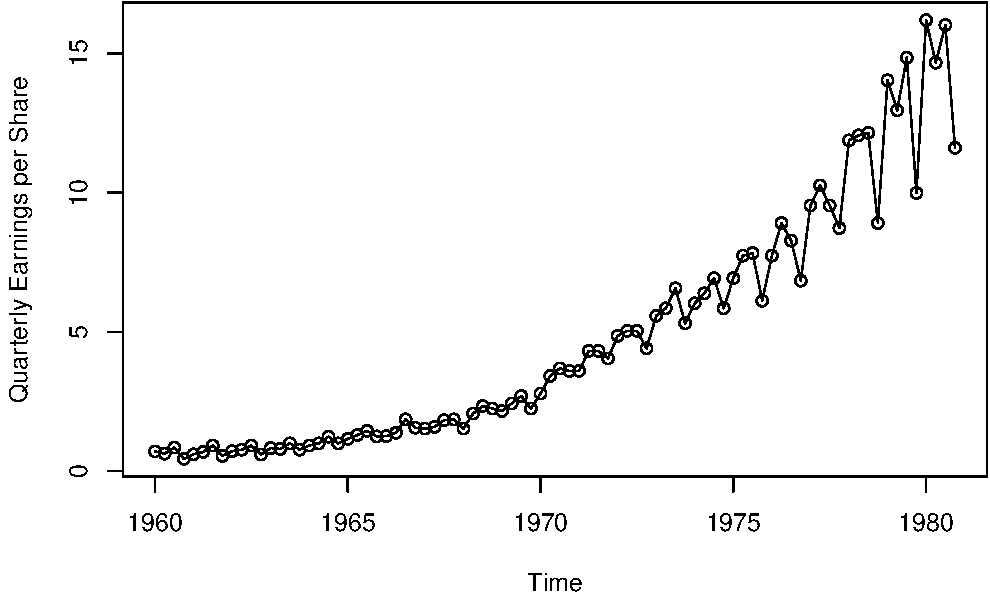
\includegraphics[width=0.75\textwidth]{jj.pdf}
    \caption{Quarterly Johnson and Johnson Earnings}\label{fig:jj}
\end{figure}
Observe that in~\Cref{fig:jj}:
\begin{itemize}
    \item The earnings are steadily increasing over time.
    \item There is heterogeneity in the variance over time.
\end{itemize}

With time series data, we are typically concerned
with the same goals as in classical statistics (prediction and inference).
However, in contrast, with time series, the data often exhibit:
\begin{enumerate}[(1)]
    \item Heterogeneity
          \begin{itemize}
              \item Time trends $ \rightarrow \E{X_t}\neq \E{X_{t+h}} $
              \item Heteroskedasticity
                    $ \rightarrow \Var{X_t}\neq \Var{X_{t+h}} $
          \end{itemize}
          {\color{blue}In classical statistics, it's assumed that all the observations have the
          same distribution which is clearly \underline{not} the case in time series.}
    \item Serial Dependence (Serial Correlation)
          \begin{itemize}
              \item Observations that are temporally close appear to depend
                    on each other.
          \end{itemize}
          {\color{blue}In classical statistics, each successive observation is assumed
          to be independent which is clearly \underline{not} the case in time series.}
\end{enumerate}

\begin{figure}[!ht]
    \centering
    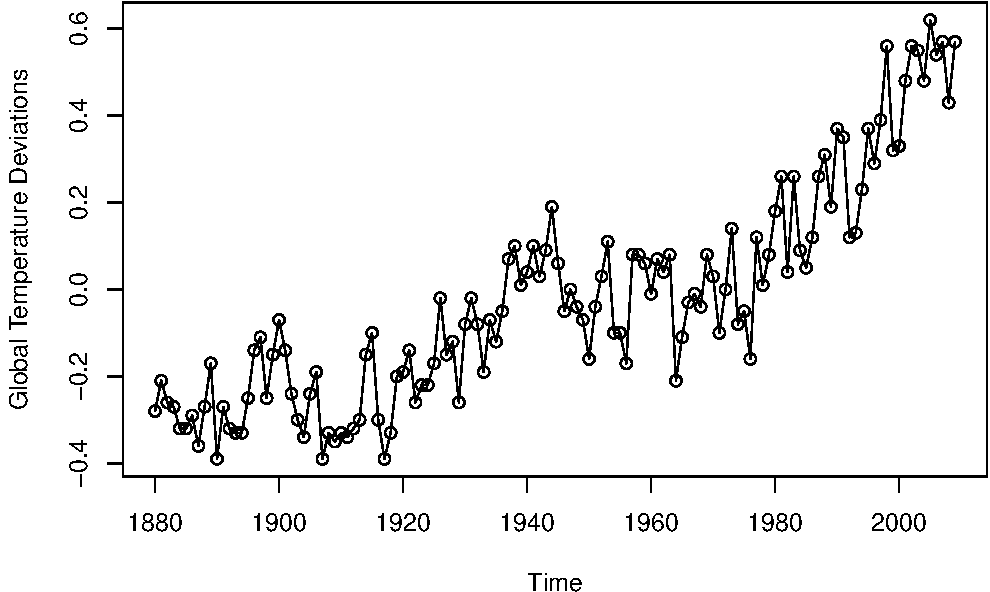
\includegraphics[width=0.75\textwidth]{gtemp.pdf}
    \caption{$ x_t $ is the deviation of global mean
        yearly temperature from the mean computed from 1951--1980}\label{fig:gtemp}
\end{figure}

Observe that in~\Cref{fig:gtemp}:
\begin{itemize}
    \item The global temperature is steadily increasing over time.
    \item There is heterogeneity in the mean over time.
    \item Heterogeneity in the variance over time is not very apparent.
    \item Serial dependence occurs.
\end{itemize}

\begin{Definition}{Time series (Formal Definition)}{}
    We say $ \set{X_t}_{t\in\mathbf{Z}} $
    is a \textbf{time series} if $ \set{X_t : t\in\mathbf{Z}} $
    is a stochastic process indexed by $ \mathbf{Z} $.
\end{Definition}
In other words, there is a common probability space
$ (\Omega,\mathcal{F},\mathbb{P}) $ so that for all
$ X_t:\Omega\to\mathbf{R} $ is a random variable.

In relation to the original definition, we say
$ X_1,\ldots,X_T $ is an \textbf{observed stretch} (\textbf{realization},
\textbf{simple path}) of length $ T $ from $ \set{X_t}_{t\in\mathbf{Z}} $.

    {\color{blue}Formally speaking, we think of a time series as being a little snippet
        of one long sample path the stochastic process for which would characterize
        all the serial dependence, time trends, and heteroskedasticity,
        that exist within a time series.}

\section{Basic Principles of Forecasting}
Consider a time series of length $ T $, namely $ X_1,\ldots,X_T $.
Based on $ X_1,\ldots,X_T $, we would like to produce a ``best guess''
for $ X_{T+h} $:
\[ \hat{X}_{T+h}=\hat{X}_{T+h\mid T}=f_h(X_T,\ldots,X_1) \]
\begin{Definition}{Forecast, Horizon}{}
    For $ h\ge 1 $, our ``best guess''
    \[ \hat{X}_{T+h}=f_h(X_T,\ldots,X_1) \]
    is called a \textbf{forecast} of $ X_{T+h} $
    at \textbf{horizon} $ h $.
\end{Definition}
There are two primary goals in forecasting:
\begin{itemize}
    \item Goal 1: Choose $ f_n $ ``optimally.'' Normally,
          we or the practitioner have some measure, say $ L(\cdot,\cdot) $,
          in mind for determining how ``close'' $ \hat{X}_{T+h} $
          is to the true value, $ X_{T+h} $. We then wish to choose $ f_h $ so that
          $ L(X_{T+h},f_h(X_T,\ldots,X_1)) $
          is minimized.

          \begin{Example}{}{}
              Most common measure $ L(\cdot,\cdot) $ is mean-squared error
              (MSE), where
              \[ L(X,Y)=\E{(X-Y)^2} \]
          \end{Example}
    \item \textbf{Goal 2}: Quantify the uncertainty in the forecast.
          This entails providing some description of how close
          we expect $ \hat{X}_{T+h} $ to be to $ X_{T+h} $.
          \begin{Example}{Why is it important to quantify uncertainty?}{}
              Suppose every minute, we flip a coin and denote
              \begin{itemize}
                  \item $ H\to 1 $
                  \item $ T\to -1 $
                  \item $ X_t= $ outcome in minute $ t $,
                        where $ t=1,\ldots,T $.
              \end{itemize}
              This produces a time series of length $ T $, which is a random
              sequence of $ (1) $'s and $ (-1) $'s. Note $ \E{X_t}=0 $.
              So, if we wish to forecast for $ h\ge 1 $,
              consider $ \hat{X}_{T+h}=f(X_T,\ldots,X_1) $
              \begin{align*}
                  L(X_{T+h},\hat{X}_{T+h})
                   & =\E{(X_{T+h}-\hat{X}_{T+h})^2}                                   \\
                   & =\E{X_{T+h}^2}+\E{\hat{X}_{T+h}^2}-2\E{X_{T+h}\hat{X}_{T+h}}     \\
                   & =\E{X_{T+h}^2}+\E{\hat{X}_{T+h}^2}-2\E{X_{T+h}}\E{\hat{X}_{T+h}} \\
                   & =\E{X_{T+h}^2}+\E{\hat{X}_{T+h}^2}
              \end{align*}
              Furthermore, note that
              $ \E{X_{T+h}^2}=\Var{X_t} $ since $ \E{X_{T+h}}=0 $.

              We can write $ \E{X_{T+h}\hat{X}_{T+h}}=\E{X_{T+h}}\E{\hat{X}_{T+h}} $ since
              $ \hat{X}_{T+h} $ is a function of the data
              $ X_T,\ldots,X_1 $, and hence independent of $ X_{T+h} $.

              We can minimize this by taking $ \hat{X}_{T+h}=0 $. There's
              nothing ``wrong'' with this forecast. But ideally,
              we would also be able to say that the sequence appears to be random,
              and that we don't expect this forecast to be close to the actual value.

                  {\color{blue}Furthermore, for this basic reason, one can always
                      argue that any forecast that's not accompanied with some
                      type of quantification of how close we expect the forecast to be,
                      is at very least hard to interpret; at worst, meaningless
                      because it doesn't
                      describe the accuracy for which we expect the forecast to perform.}
          \end{Example}
\end{itemize}
How can we quantify the uncertainty in forecasting?

Ideal: The predictive distribution:
\[ X_{T+h}\mid X_T,\ldots,X_1 \]
Excellent: Predictive intervals/sets. For some $ \alpha\in(0,1) $
find $ I_\alpha $ so that
\[ \Prob{X_{T+h}\in I_\alpha\given X_T,\ldots,X_1}=\alpha \]
($ \alpha=0.95 $, for example). Often such intervals take the form
\[ I_\alpha=(\hat{X}_{T+h}-\hat{\sigma}_h,\hat{X}_{T+h}+\hat{\sigma}_h) \]
Concluding remarks:
\begin{enumerate}
    \item Estimating predictive distribution leads one towards
          estimating the joint distribution of
          \[ X_{T+h},X_T,\ldots,X_1 \]
          For example, ARMA and ARIMA models.
    \item It is important that we acknowledge that some things cannot be predicted!
\end{enumerate}
``It is tough to make predictions, especially about the future.''---Yogi Berra

\section{Definitions of Stationary}
Given a time series $ X_1,\ldots,X_T $, we are
frequently interested in estimating the joint distribution of
\[ X_{T+h},X_T,\ldots,X_1 \]
which is useful for forecasting and inference.

The joint distribution is a feature of the process
$ \set{X_{t}}_{t\in\mathbf{Z}} $
\[ X_1,\ldots,X_T\xrightarrow[\text{infer}]{}\set{X_t}_{t\in\mathbf{Z}} \]
\begin{itemize}
    \item $ X_1,\ldots,X_T $: Observed data.
    \item $ \set{X_t}_{t\in\mathbf{Z}} $: Stochastic process.
\end{itemize}

Worst case: $ X_t\sim F_t $, where $ F_t $ is a \emph{changing}
function of $ t $. If so, it is hard to pool the data
$ X_1,\ldots,X_T $, to estimate $ F_t $. If
\textbf{serial dependence} occurs; that is, if the
distribution of $ (X_t,X_{t+h}) $
depends strongly on $ t $, then we have a similar problem in estimating
e.g.\ $ \Cov{X_t,X_{t+h}} $.

\begin{Definition}{Strictly stationary}{}
    We say that a time series $ \set{X_t}_{t\in\mathbf{Z}} $
    is \textbf{strictly stationary} (\textbf{strongly stationary})
    if for each $ k\ge 1 $, $ i_1,\ldots,i_k,h\in\mathbf{Z} $,
    \[ (X_{i_1},\ldots,X_{i_k})\stackrel{\text{d}}{=}
        (X_{i_{1}+h},\ldots,X_{i_k+h}) \]
    {\color{blue}If we look at the $ k $-dimensional joint distribution
    $ (X_{i_1},\ldots,X_{i_k}) $
    of the series at points $ i_1,\ldots,i_k $, then
    strict stationary means this is shift-invariant.}
    That is, shifting the window on which
    you view the data, does \underline{not} change its distribution.
    This implies that if $ F_t=\text{CDF} $ of $ X_t $, then
    $ F_t=F_{t+h}=F $
    that is, all variables have a common distribution function.
\end{Definition}
\begin{Definition}{Mean function}{}
    For a time series $ \set{X_t}_{t\in\mathbf{Z}} $, with
    $ \E{X_t^2}<\infty $ for all $ t\in\mathbf{Z} $,
    we denote the \textbf{mean function} of the time series as
    \[ \mu_t=\E{X_t} \]
\end{Definition}
\begin{Definition}{Autocovariance function, Lag}{}
    The \textbf{autocovariance} function of the time series $ \set{X_t}_{t\in\mathbf{Z}} $
    is defined as
    \[ \gamma(t,s)=\E{(X_t-\mu_t)(X_s-\mu_s)}=\Cov{X_t,X_s} \]
\end{Definition}
\begin{Definition}{Weakly stationary, Lag}{}
    We say that a time series $ \set{X_t}_{t\in\mathbf{Z}} $
    is \textbf{weakly stationary} if $ \E{X_t}=\mu $
    (does not depend on $ t $), and if
    \[ \gamma(t,s)=f(\abs{t-s}) \]
    that is, $ \gamma(t,s) $ is a function of $ \abs{t-s} $. In this case,
    we usually write
    \[ \gamma(h)=\Cov{X_t,X_{t+h}} \]
    and we call the input $ h $ the \textbf{lag} parameter.
\end{Definition}
Additional terminology:
\begin{itemize}
    \item The property when $ \E{X_t}=\mu $ does not depend
          on $ t $ is often called the \textbf{first order stationary}.
    \item The property when $ \gamma(t,s)=\gamma(\abs{t-s}) $
          only depends on the lag $ \abs{t-s} $ is called the
          \textbf{second order stationary}.
    \item For a second order stationary process,
          \begin{align*}
              \gamma(h)
               & =\Cov{X_t,X_{t+h}}                                      \\
               & =\Cov{X_{t-h},X_{t-h+h}} & \quad & t\rightarrow{} (t-h) \\
               & =\Cov{X_t,X_{t-h}}                                      \\
               & =\gamma(-h)
          \end{align*}
          Since $ \gamma(h)=\gamma(-h) $, we
          normally, we only record $ \gamma(h) $ for $ h\ge 0 $.
\end{itemize}
\section{White Noise and Stationary Examples}
\begin{Definition}{Strong white noise}{}
    We say $ \set{X_t}_{t\in\mathbf{Z}} $ is a
    \textbf{strong white noise} if $ \E{X_t}=0 $
    and the $ \set{X_t}_{t\in\mathbf{Z}} $ are i.i.d.
\end{Definition}
\begin{Definition}{Weak white noise}{}
    We say $ \set{X_t}_{t\in\mathbf{Z}} $ is a
    \textbf{weak white noise} if $ \E{X_t}=0 $
    and
    \[ \gamma(t,s)=\Cov{X_t,X_s}=\begin{cases}
            \sigma^2 & \abs{t-s}=0 \\
            0        & \abs{t-s}>0
        \end{cases} \]
\end{Definition}
\begin{Definition}{Gaussian white noise}{}
    We say $ \set{X_t}_{t\in\mathbf{Z}} $ is a
    \textbf{Gaussian white noise}
    if $ X_t\stackrel{\text{iid}}{\sim}\N{0,\sigma^2} $.
\end{Definition}
\begin{figure}[!ht]
    \centering
    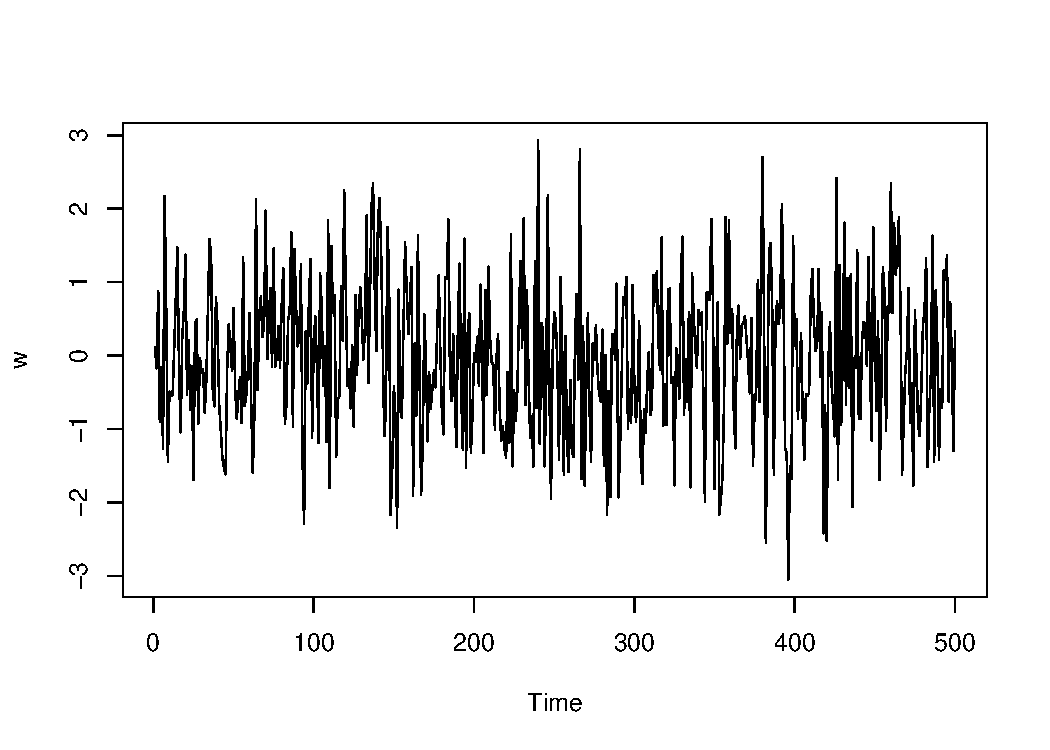
\includegraphics[width=0.75\textwidth]{wn.pdf}
    \caption{Gaussian White Noise of Length 500}\label{fig:wn}
\end{figure}
Figure~\ref{fig:wn} is a Gaussian \emph{white} noise series.
\textbf{White} comes from spectral analysis,
in which a white noise series shares the same spectral properties as white light:
all periodicities occur with equal strength.
\begin{Example}{}{}
    Suppose $ \set{W_t}_{t\in\mathbf{Z}} $
    is a strong white noise, then $ \E{W_t}=0 $;
    that is, it doesn't depend on $ t $.
    \[ \gamma(t,s)=\Cov{W_t,W_s}=\E{W_t W_s}=
        \begin{cases}
            \sigma_W^2 & \abs{t-s}=0 \\
            0          & \abs{t-s}>0
        \end{cases} \]
    only depends on $ \abs{t-s} $.

    $ \set{W_t}_{t\in\mathbf{Z}} $ is
    \textbf{weakly stationary}. Furthermore,
    $ \set{W_t}_{t\in\mathbf{Z}} $ is
    \textbf{strictly stationary}. Let $ k\ge 1 $
    with $ i_1<\cdots i_k $ and $ h\in\mathbf{Z} $, then
    \begin{align*}
        \Prob{W_{i_1}\le t_1,\ldots,W_{i_k}\le t_k}
         & =\prod_{j=1}^k\Prob{W_{i_j}\le t_j}                   & \quad & \text{independence} \\
         & =\prod_{j=1}^k\Prob{W_{{i_j}+h}\le t_j}                                             \\
         & =\Prob{W_{{i_1}+h}\le t_1,\ldots, W_{{i_k}+h}\le t_k}
    \end{align*}
\end{Example}
\begin{Example}{}{}
    Suppose $ \set{W_t}_{t\in\mathbf{Z}} $ is a strong white noise.
    Define $ X_t=W_t+\theta W_{t-1} $ for $ \theta\in\mathbf{R} $.
    Since $ \set{W_t}_{t\in\mathbf{Z}} $ is a strong white noise, we
    have $ \E{W_t}=0 $ for all $ t $, and so we
    have $ \E{X_t}=\E{W_t+\theta W_{t-1}}=\E{W_t}+\theta\E{W_{t-1}}=0 $
    which is first order stationary.
    \[ \gamma(t,s)=\Cov{X_t,X_s}=\begin{cases}
            (1+\theta^2)\sigma_W^2 & \abs{t-s}=0 \\
            \theta\sigma_W^2       & \abs{t-s}=1 \\
            0                      & \abs{t-s}>0
        \end{cases} \]
    We obtain these calculations as follows:
    \begin{itemize}
        \item $ \abs{t-s}=0 $.
              \[ \E{(W_t+\theta W_{t-1})^2}
                  =\E{W_t^2}+\theta^2\E{W_{t-1}^2}+2\E{\theta W_t W_{t-1}}
                  =(1+\theta^2)\sigma_W^2 \]
        \item $ t=s+1 $ (or $ s=t+1 $).
              \[ \E{(W_{s+1}+\theta W_s)(W_s+\theta W_{s-1})}=\theta\E{W_s^2}=\theta\sigma_W^2 \]
              since $ W_{s+1} $ is independent of $ W_s $ and $ W_{s-1} $.
              The calculation is easy to verify.
        \item $ \abs{t-s}>1 $. $ W_t+\theta W_{t-1} $ is independent of
              $ W_s+\theta W_{s-1} $.
    \end{itemize}
    $ \set{X_t}_{t\in\mathbf{Z}} $ is also strictly stationary.
    Suppose $ k\ge 1 $, $ i_1,\ldots,i_k, h\in\mathbf{Z} $
    with $ i_1<\cdots<i_k $, then
    \begin{align*}
        \Prob{X_{i_1}\le t_1,\ldots,X_{i_k}\le t_k}
         & =\Prob{W_{i_1}+\theta W_{{i_1}-1}\le t_1,\ldots,W_{i_k}+\theta W_{{i_k}-1}\le t_k} \\
         & =\Prob*{\begin{bmatrix}
                W_{{i_1}-1} \\
                W_{i_1}     \\
                \vdots      \\
                W_{i_k}
            \end{bmatrix}\in B}                                           \\
         & =\Prob*{\begin{bmatrix}
                W_{{i_1-1}+h} \\
                \vdots        \\
                W_{{i_k}+h}
            \end{bmatrix}\in B}                                           \\
         & =\Prob{X_{{i_1}+h}\le t_1,\ldots,X_{{i_k}+h}\le t_k}
    \end{align*}
    where $ B $ is some subset of $ \mathbf{R}^{i_k-i_1+1} $, and hence
    is shift-invariant.
\end{Example}
\begin{Definition}{Bernoulli shift}{}
    Suppose $ \set{\varepsilon_t}_{t\in\mathbf{Z}} $ is a
    strong white noise. If $ X_t=g(\varepsilon_t,\varepsilon_{t-1},\ldots) $
    for some function $ g:\mathbf{R}^\infty \to \mathbf{R} $, we say that
    $ \set{X_t}_{t\in\mathbf{Z}} $ is a \textbf{Bernoulli shift}.
\end{Definition}
\begin{Theorem}{}{}
    If $ \set{X_t}_{t\in\mathbf{Z}} $ is a Bernoulli shift, then
    $ \set{X_t}_{t\in\mathbf{Z}} $ is strictly stationary.
\end{Theorem}
\begin{Remark}{}{}
    Norbert Wiener conjectured that \textbf{every} stationary
    sequence is a Bernoulli shift, which is not true. The truth is,
    almost every one is.
\end{Remark}
\begin{Exercise}{}{}
    Suppose $ \set{W_t}_{t\in\mathbf{Z}} $ is a strong white noise.
    The \textbf{two-sided random walk} is defined as
    \[ X_t=\sum_{i=0}^{t} W_i+\sum_{i=t}^{-1} W_i  \]
    Show that $ \set{X_t}_{t\in\mathbf{Z}} $ is first order stationary,
    but $ \set{X_t}_{t\in\mathbf{Z}} $ is \underline{not} second order stationary.
\end{Exercise}
\section{Weak versus Strong Stationary}
Sadly, $ \set{X_t}_{t\in\mathbf{Z}} $ is strictly stationary does \underline{not} imply
$ \set{X_t}_{t\in\mathbf{Z}} $ is weakly stationary.
\begin{Example}{}{}
    Suppose $ X_t\stackrel{\text{iid}}{\sim} $ Cauchy Random Variables;
    that is,
    \[ \Prob{X_t\le s}=\int_{-\infty}^{s} \frac{1}{\pi(1+x^2)}\, d{x}  \]
    Then, $ \E{X_t} $ does not exist, and hence $ \set{X_t}_{t\in\mathbf{Z}} $ cannot
    be weakly stationary. However, $ \set{X_t}_{t\in\mathbf{Z}} $ is strictly
    stationary in this case since $ \set{X_t}_{t\in\mathbf{Z}} $ is a strong
    white noise.
\end{Example}
\begin{Theorem}{}{strongly_imp_weakly}
    If $ \set{X_t}_{t\in\mathbf{Z}} $ is strongly stationary and $ \E{X_0^2}<\infty $,
    then $ \set{X_t}_{t\in\mathbf{Z}} $ is weakly stationary.
\end{Theorem}
\begin{Proof}{\Cref{thm:strongly_imp_weakly}}{}
    Note that if $ \set{X_t}_{t\in\mathbf{Z}} $ is strictly stationary,
    \[ (X_t)\stackrel{\text{d}}{=}(X_0) \]
    so that $ \E{X_t}=\E{X_0} $ which does not depend on $ t $, and also
    \[ \Var{X_t}=\Var{X_0} \]
    By the Cauchy-Schwarz inequality,
    \[ \gamma(t,s)=\Cov{X_t,X_s}\le \Var{X_t}<\infty \]
    and suppose $ t<s $,
    \[ \Cov{X_t,X_s}=\Cov{X_0,X_{s-t}}=f(\abs{s-t}) \]
    since it is shift-invariant, and hence if we shift everything over by $ t $,
    \[ (X_t,X_s)\stackrel{\text{d}}{=}(X_{t-t},X_{s-t})\stackrel{\text{d}}{=}(X_0,X_{s-t}) \]
\end{Proof}
\begin{Definition}{Gaussian process}{}
    $ \set{X_t}_{t\in\mathbf{Z}} $ is said to be a
    \textbf{Gaussian process} (\textbf{Gaussian time series}) if
    for each $ k\ge 1 $, $ i_1<i_2<\cdots<i_k $ we have
    \[ (X_{i_1},\ldots,X_{i_k})\sim
        \Mvn{\symbf{\mu}_k(i_1,\ldots,i_k),\symbf{\Sigma}_{k\times k}(i_1,\ldots,i_k)} \]
    \[ \symbf{\mu}_k=\begin{bmatrix}
            \E{X_{i_1}} \\
            \vdots      \\
            \E{X_{i_k}}
        \end{bmatrix}\quad
        \symbf{\Sigma}_{k\times k}=
        \Cov{X_{i_j},X_{i_r}}_{1\le j,\, r\le k} \]
\end{Definition}
\begin{Theorem}{}{weak_gaussian_imp_strictly}
    If $ \set{X_t}_{t\in\mathbf{Z}} $ is weakly stationary and a Gaussian process, then
    $ \set{X_t}_{t\in\mathbf{Z}} $ is strictly stationary.
\end{Theorem}
\begin{Proof}{\Cref{thm:weak_gaussian_imp_strictly}}{}
    If $ \set{X_t}_{t\in\mathbf{Z}} $ is weakly stationary, then $ \E{X_t}=\mu $ for all $ t $.
    \[ (X_{i_1},\ldots,X_{i_k})\rightarrow
        \begin{bmatrix}
            \E{X_{i_1}} \\
            \vdots      \\
            \E{X_{i_k}}
        \end{bmatrix}=\begin{bmatrix}
            \mu    \\
            \vdots \\
            \mu
        \end{bmatrix}=\symbf{\mu}=
        \begin{bmatrix}
            \E{X_{{i_1}+h}} \\
            \vdots          \\
            \E{X_{{i_k}+h}}
        \end{bmatrix} \]
    Also,
    \begin{align*}
        \Var{X_{i_1},\ldots,X_{i_k}}
         & =\Cov{X_{i_j},X_{i_r}}_{1\le j,\, r\le k} \\
         & =\Cov{X_0,X_{i_r-i_j}}_{1\le j,\, r\le k} \\
         & =\Cov{X_0,X_{i_r+h},X_{i_r+h-(i_j+h)}}    \\
         & =\Cov{X_{i_j+h},X_{i_r+h}}                \\
         & =\Var{X_{i_1+h},\ldots,X_{i_k+h}}
    \end{align*}
\end{Proof}
\begin{Example}{}{}
    Using the Gaussian assumption
    \[ (X_{i_1},\ldots,X_{i_k})
        \stackrel{\text{d}}{=}\Mvn{\symbf{\mu},\symbf{\Sigma}_{k\times k}}
        \stackrel{\text{d}}{=}(X_{i_1+h},\ldots,X_{i_k+h}) \]
    Hence $ \set{X_{t}}_{t\in\mathbf{Z}} $ is strictly stationary
    in this case.
\end{Example}
\begin{Exercise}{}{}
    Prove that if $ \set{X_t}_{t\in\mathbf{Z}} $ is \underline{not}
    weakly stationary; that is, either $ \E{X_t} $ depends on $ t $
    or $ \gamma(t,s) $ does not depend on the lag,
    then $ \set{X_t}_{t\in\mathbf{Z}} $ is \underline{not} strictly stationary.
\end{Exercise}

\section{\texorpdfstring{$ \dagger $}{†} Theoretical L2 Framework for Time Series}
\begin{itemize}
    \item $ X_t = \lim\limits_{{h} \to {\infty}} X_{h,t} $. In what sense
          does this limit exist?
    \item How ``close'' are two random variables $ X $ and $ Y $?
    \item Is there a random variable that achieves
          \[ \inf_{y\in S}d(Y,S) \]
\end{itemize}
\begin{Definition}{$ L^2 $ space}{}
    Consider a probability space $ (\Omega,\mathcal{F},\mathbb{P}) $.
    The space $ L^2 $ is the set of random variables
    $ X:\Omega\to\mathbf{R} $ measurable so that $ \E{X^2}<\infty $.
\end{Definition}
\begin{Definition}{$ L^2 $-time series}{}
    We say that $ \set{X_t}_{t\in\mathbf{Z}} $ is
    and $ L^2 $-time series if $ X_t\in L^2 $ for all
    $ t\in\mathbf{Z} $.
\end{Definition}
$ L^2 $ is a Hilbert space when equipped
with inner product, $ X,Y\in L^2 $.
\[ \innerp{X}{Y}=\E{XY} \]
$ \innerp{}{} $ is an inner product since it is
\begin{enumerate}[(1)]
    \item Linear: $ \innerp{aX+bY}{Z}=a\innerp{X}{Z}+b\innerp{Y}{Z} $.
    \item ``Almost'' Positive Definite:
          $ \innerp{X}{X}=\E{X^2}=0 \iff X=0 $ almost surely.
          Which implies $ \Prob{X=0}=1 $.
    \item Symmetric: $ \innerp{X}{Y}=\innerp{Y}{X} $.
\end{enumerate}
$ L^2 $ is complete with this inner product; that is,
whenever $ X_n\in L^2 $ so that $ \E{(X_n-X_m)^2}\to 0 $
as $ n,m\to\infty $, then there exists $ X\in L^2 $
so that $ X_n\to X $; that is, $ \E{(X_n-X)^2}\to 0 $.
This follows from the ``famous'' Riesz-Fischer Theorem.
\subsection{Useful Tools for Time Series}
\begin{enumerate}[(1)]
    \item \textbf{Existence of Limits}
          \[ X_{t,n}=\sum_{j=0}^{n} \Psi_j \varepsilon_{t-j}
          \]
          $ \set{\varepsilon_t}_{t\in\mathbf{Z}} $ is a strong white noise.
          Since for $ n>m $,
          \[ \E{(X_{t,n}-X_{t,m})^2}
              =\E[\bigg]{\biggl(\sum_{j=m+1}^{n} \Psi_j \varepsilon_{t-j}\biggr)^{\!2}}
              =\sum_{j=m+1}^{n} \Psi_j^2\sigma_{\varepsilon}^2\to 0\text{ as }
              n,m\to \infty \]
          only if $ \sum_{j=0}^{\infty} \Psi_j^2<\infty $, then there \textbf{must}
          exist a random variable $ X_t $ (by the completeness of $ L^2 $), so that
          \[ X_t=\lim\limits_{{n} \to {\infty}} X_{t,n}=\sum_{j=0}^{\infty}
              \Psi_j \varepsilon_{t-j} \]
    \item \textbf{Projection Theorem and Forecasting}.
          Forecasting can be often cast as finding a random variable $ Y $ among
          a collection of possible forecasts $ \mathcal{M} $ (e.g.
          $ \mathcal{M}=\Span{X_T,\ldots,X_1} $) so that
          \[ Y={\arg\inf}_{Z\in\mathcal{M}}\E{(X_{T+h}-Z)^2} \]
          When $ \mathcal{M} $ is a closed linear subspace of $ L^2 $,
          the Projection Theorem guarantees that such a $ Y $ exists,
          and it must satisfy
          \[ \innerp{X_{T+h}-Y}{Z}=0\quad\forall Z\in\mathcal{M} \]
          must be in the orthogonal complement.
\end{enumerate}

\section{Signal and Noise Models}
``Ideally,'' a time series that we are considering
was generated from a stationary process. If so,
we can pool data to estimate the processes underlying structure
(e.g.\ its marginal distribution and serial dependence structure)

Most time series are evidently \underline{not} stationary.

Looking back at Figure~\ref{fig:jj}:
\begin{itemize}
    \item Mean appears to increase, so it is not first order stationary;
    \item Variability also appears to increase, so it is not
          second order stationary;
    \item Therefore, it is not strictly stationary.
\end{itemize}
Signal and Noise Model: $ X_t=S_t+\varepsilon_t $
\begin{itemize}
    \item $ S_t $ is the \textbf{deterministic}
          ``signal'' or ``trend'' of the series
    \item $ \varepsilon_t $ is the ``noise'' added
          to the signal satisfying $ \E{\varepsilon_t}=0 $, hence
          $ \E{X_t}=\E{S_t+\varepsilon_t}=\E{S_t} $.
          There exists a (strong) white noise $ \set{W_t}_{t\in\mathbf{Z}} $
          so that
          \[ \varepsilon_t=g(W_t,W_{t-1}\ldots,)\quad\text{[Stationary Noise]} \]
          \[ \varepsilon_t=g_t(W_t,W_{t-1}\ldots,)\quad\text{[Non-stationary Noise]} \]
          The terms $ \set{W_t}_{t\in\mathbf{Z}} $ are often called the
          ``innovations'' or ``shocks'' during the random behaviour
          of $ X_t $.

              {\color{blue}$ g $ is used to try to capture noise that can
                  potentially have serial dependence.}
\end{itemize}
\begin{Example}{}{}
    An example of a function $ g $ so that $ \varepsilon_t=g_t(W_t,W_{t-1},\ldots) $
    might be a \textbf{random walk}; that is, $ \varepsilon_t=\sum_{j=0}^{t} W_j $.
    Another example could be the \textbf{changing variance models}; that is,
    $ \varepsilon_t=\sigma(t)W_t $.
\end{Example}
Our goal is to estimate $ S_t $, and then infer the structure of $ \varepsilon_t $.

In Figure~\ref{fig:gtemp}, the model appears to be non-stationary
(trending upwards over time),
so we might try the signal and noise model. We might posit
a linear trend, or even higher order functions.

For the temperature data, we may posit that
\[ S_t=\beta_0+\beta_1 t\quad\text{[Linear Trend]} \]
The trend may be estimated by ordinary least squares (OLS).
We choose $ \beta_0 $ and $ \beta_1 $ to minimize
\[ \sum_{t=1}^{T} \bigl[X_t-(\beta_0+\beta_1 t)\bigr]^2 \]
This can be done in R using the \code{lm()} command, and
can easily be computed with calculus. Figure~\ref{fig:gtemp_lm}
is a small example of the global temperature data superimposed
with \code{lm()}'s estimate.
\begin{figure}[!ht]
    \centering
    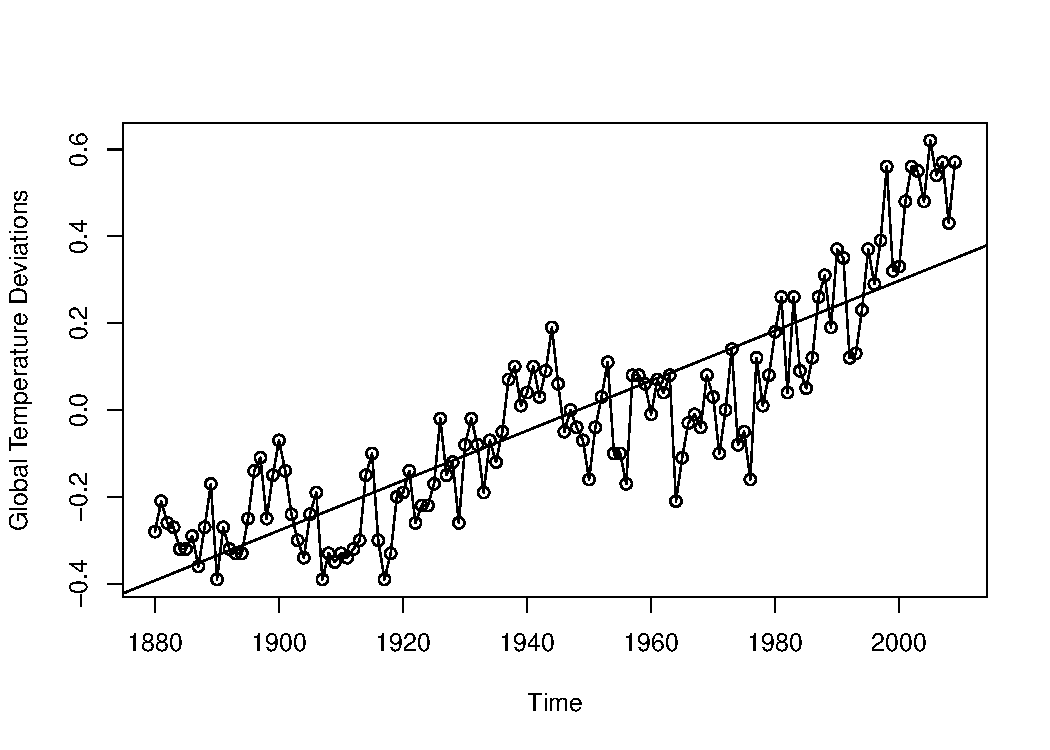
\includegraphics[width=0.75\textwidth]{gtemp_lm.pdf}
    \caption{OLS estimate of a linear trend.}\label{fig:gtemp_lm}
\end{figure}
Let's introduce some terminology about trends.
\begin{Definition}{Detrended time series}{}
    Detrending a time series constitutes computing the
    residuals based on an estimate for the signal/trend.

    A \textbf{detrended time series} is a time series of such residuals.
    \begin{enumerate}
        \item Estimate $ S_t\to \hat{S_t} $
        \item Detrend series: $ X_t-\hat{S_t}=Y_t $
              where $ Y_t $ is the ``detrended'' series.
    \end{enumerate}
\end{Definition}

If the trend is zero, there appears to be a substantial serial
dependence remaining in the time series.

\section{Time Series Differencing}
Signal and Noise Model: $ X_t=S_t+\varepsilon_t $. Hopefully,
upon estimating $ S_t $ with $ \hat{S}_t $,
we find $ X_t-\hat{S}_t=\hat{\varepsilon}_t $ (detrended series)
looks reasonably stationary. If the residuals would be
reasonably stationary, we might
proceed in estimating their underlying structure of $ \set{\hat{\varepsilon}_t}_{t=1,\ldots,T} $.
as if it were stationary. {\color{blue}In particular, we might try to estimate their marginal
        distributions and/or their serial dependence structure. If we thought those estimates
        were reasonably good, we would have a good idea of how the time series $ X_t $ behaves.}

\textbf{Random Walk with Drift Model}. Let $ \varepsilon_t $ be a strong white noise.
\begin{align*}
    X_t
     & =\delta+X_{t-1}+\varepsilon_t                                                                                  \\
     & =\delta+\delta+X_{t-2}+\varepsilon_{t-1}+\varepsilon_t                                                         \\
     & =\delta+\delta+\delta+X_{t-3}+\varepsilon_{t-2}+\varepsilon_{t-1}+\varepsilon_{t}                              \\
     & \vdots                                                                            & \quad & \text{$ t $ times} \\
     & =t\delta+X_0+\sum_{j=1}^{t} \varepsilon_j
\end{align*}
where we note that $ t\delta+X_0=S_t $ is a linear signal,
and $ \sum_{j=1}^{t} \varepsilon_j $ is a
random walk noise.

Notice that under the Random Walk Model.
\[ X_t-X_{t-1}=\nabla X_t=\delta+\varepsilon_t \]
So, if $ X_t $ follows a random walk model, the series $ Y_t=\delta X_t $
should behave like a white noise shifted by $ \delta $.

\begin{Definition}{Differenced time series}{}
    Differencing a time series constitutes
    computing the difference between successive terms.

    A \textbf{differenced time series} is a time series of such differences.
    The first differenced series is denoted
    \[ \nabla X_t=X_t-X_{t-1} \]
    and is the series of length $ T-1 $, namely
    \[ X_2-X_1,X_3-X_2,\ldots,X_T-X_{T-1} \]
    Higher order differences are calculated recursively, so
    \[ \nabla^d X_t=\nabla^{d-1}\nabla X_t \]
    where $ \nabla^d $ is the $ d^{\text{th}} $ order difference and
    we define $ \nabla^0 X_t=X_t $.
\end{Definition}

Detrending and Differencing are both ways of reducing a
(potentially non-stationary) time series
to an approximately stationary series.

\underline{Differencing vs. Detrending}

\emph{Pros}:
\begin{itemize}
    \item Differencing does not require the parameter estimation
          (don't need to estimate $ S_t $).
    \item Higher order differencing can reduce even very
          ``trendy'' series to look more like noise.
\end{itemize}
\emph{Cons}:
\begin{itemize}
    \item Differencing can ``wash away'' features of the series,
          and introduce more complicated structures.
    \item The trend is often of interest, and good estimates
          of the trend lead to improved long-range forecasts.
\end{itemize}
\begin{Example}{Differencing can complicate time series}{}
    $ X_t=W_t $ where $ W_t $ is a strong white noise.
    \[ \nabla X_t=W_t-W_{t-1}=Y_t \]
    \[ \gamma_X(h)=\Cov{X_t,X_{t+h}}=\begin{cases}
            \sigma_W^2 & h=0    \\
            0          & h\ge 1
        \end{cases} \]
    More complicated:
    \[ \gamma_Y(h)=\Cov{Y_t,Y_{t+h}}=\begin{cases}
            2\sigma_W^2 & h=0    \\
            -\sigma_W^2 & h=1    \\
            0           & h\ge 2
        \end{cases} \]
\end{Example}

\section{Sequences and Their Limits}
\subsection{Introduction to Subsequences}
\begin{Definition}{}{}
    An infinite sequence of numbers is a list of numbers in a definite order, e.g.,
    \[ a_1,a_2,a_3,a_4,\ldots,a_n,\; a_i\in\R. \]
    \underline{Notation}: $ \Set{a_1,a_2,\ldots,a_n} $ or $ \sequence{a_n}_{n=1}^{\infty} $ or $ \sequence{a_n} $.
\end{Definition}
Sequences can be defined explicitly (in terms of $ n $) or recursively (in terms of previous terms).
\begin{Example}{Explicit Sequences}{}
    \begin{itemize}
        \item $ \Set*{\frac{1}{n+1}}_{n=1}^{\infty} $: $ 1/2,1/3,1/4,1/5,\ldots $.
        \item $ \Set{\sqrt{n+2}}_{n=2}^{\infty} $: $ \sqrt{4},\sqrt{5},\sqrt{6},\ldots $.
        \item $ \Set{(-1)^n}_{n=1}^\infty $: $ -1,1,-1,1,\ldots $.
    \end{itemize}
\end{Example}
\subsection{Recursively Defined Sequences}
\begin{Example}{Recursive Sequences}{}
    \begin{itemize}
        \item $ a_1=1 $, $ a_{n+1}=\sqrt{1+a_n} $, so $ a_1=1 $, $ a_2=\sqrt{2} $, $ a_3=\sqrt{1+\sqrt{2}} $, and so on for $ n\ge 1 $.
        \item Fibonacci's sequence: $ a_1=1 $, $ a_2=1 $, $ a_{n+2}=a_{n+1}+a_n $ for $ n\ge 1 $, i.e.,
              $ 1,1,2,3,5,8,13,\ldots $.
    \end{itemize}
\end{Example}
We can plot sequences on a number line, or we could think of a sequence as a function $ f\colon \N\to\R $, writing $ f(n)=a_n $, e.g.,
for $ a_n=1/2 $ we would write $ f(n)=1/2 $.

\underline{Why study sequences?}
\begin{itemize}
    \item Lots of continuous processes can be modelled with discrete data, as we will see.
    \item We can use recursive sequences to approximate solutions to equations that can't be solved explicitly (Newton's Method).
    \item For another (ancient) application, see page 14 of the course notes about calculating square roots.
\end{itemize}
Our goal now will be to determine how to find the limit of a sequence, that is, find what the value of the terms of the sequence
are approaching (if it exists).

We may want to build new sequences out of old ones or only discuss what happens to a sequence eventually, that is, after a certain index.
\begin{Example}{}{}
    For $ \Set{\frac{1}{n}}_{n=1}^{\infty} $, if we consider only the odd terms, we get $ 1,1/3,1/5 $, or the $ k\textsuperscript{th} $
    term is
    \[ \frac{1}{2k-1} \]
    for $ k\in\N $.
    This is called a subsequence.
\end{Example}
\subsection{Subsequences and Tails}
\begin{Definition}{Subsequence}{}
    If $ \sequence{a_n} $ is a sequence and $ {n_1,n_2,\ldots} $ is a sequence of natural numbers, where
    $ n_1<n_2<n_3<\cdots $, then the sequence
    \[ \Set{a_{n_1},a_{n_2},\ldots}=\sequence{a_{n_k}} \]
    is a \textbf{subsequence} of $ \sequence{a_n} $.
\end{Definition}
One particular subsequence is $ \Set{a_k,a_{k+1},a_{k+2}} $ for some $ k\in\N $.
This is called the tail of $ \sequence{a_n} $ with cut-off $ k $.

\subsection{Limits of Sequences}
We are going to see lots of different limits this term, but we will start with sequences.
\begin{Example}{}{}
    $ \sequence{\frac{1}{n}} $ seems like it converges to $ 0 $, or that $ 0 $ is the limit of the sequence.
    We saw this when we plotted the sequence. We will eventually want a formal definition, but let's start intuitively.
\end{Example}
Given a sequence $ \sequence{a_n} $, what does it mean to say that $ \sequence{a_n} $ converges to $ L $
as $ n $ goes to infinity?

What about ``as $ n $ gets larger, $ a_n $ gets closer to $ L $?'' Unfortunately, this isn't a good definition. For example, as $ n $
gets larger $ \frac{1}{n} $ gets closer to $ 0 $, but it also gets closer to $ -1 $, $ -2 $, and so on. But, $ 0 $
is \underline{the} limit! What makes it different? Well, the sequence gets infinitely close to $ 0 $,
unlike the other numbers! Let's try to define this again: ``the limit of $ \sequence{a_n} $ is $ L $
if, as $ n $ gets infinitely large, $ a_n $ gets infinitely close to $ L $.'' This is much better!
But how can we formalize the idea of ``infinitely close?''
\begin{Definition}{Formal Definition of the Limit of a Sequence I}{}
    Let $ \sequence{a_n} $ be a sequence in $ \R $. For $ L\in\R $, we say that the sequence $ \sequence{a_n} $ \textbf{converges} to $ L $
    (or that the \textbf{limit} of $ \sequence{a_n} $ is equal to $ L $), and we write $ a_n\to L $ (as $ n\to\infty $), or we write
    $ \lim\limits_{{n} \to {\infty}}a_k=L $, when
    \[ \forall \varepsilon\in\R_{>0}: \exists N\in \R_{>0}:\forall n\in\N:n\ge N\implies \abs{a_n-L}<\varepsilon. \]
    We say that the sequence $ \sequence{a_n} $ \textbf{diverges to infinity}
    (in $ \R $) when there exists $ L\in \R $ such that $ \sequence{a_n} $ converges to $ L $.
    We say that the sequence \textbf{diverges} (in $ \R $) when it does not converge (to any $ L\in\R $).
\end{Definition}
\begin{Example}{}{}
    Consider $ a_n=\frac{1}{n^2} $. We'd guess that the limit is $ 0 $. Say $ \varepsilon=\frac{1}{100} $, can we find a large enough $ n\in N $
    so that $ \abs*{\frac{1}{n^2}-0}<\frac{1}{100}  $ if $ n\ge N $? Well, we need
    \[ \abs*{\frac{1}{n^2}-0}<\frac{1}{100}\implies \frac{1}{n^2}<\frac{1}{100}\implies n^2>100, \]
    so $ n>10 $. Let $ N=11 $, then if $ n\ge N $, we get
    $ \abs*{\frac{1}{n^2}-0}<\frac{1}{100} $. But wait! We aren't done yet! The definition says we need to prove it for any $ \varepsilon>0 $,
    but we only proved it for $ \varepsilon=\frac{1}{100} $. Let's adapt the proof to work for any $ \varepsilon>0 $.
\end{Example}
\underline{Proof that $ \lim\limits_{{n} \to {\infty}}\frac{1}{n^2}=0 $}.
Let $ \varepsilon>0 $ be given. Let $ N>\frac{1}{\sqrt{\varepsilon}} $ for $ N\in \N $. Then, if $ n\ge N $,
we get
\[ \abs*{\frac{1}{n^2}-0}=\frac{1}{n^2}\le \frac{1}{N^2}<\frac{1}{(1/\sqrt{\varepsilon})^2}=\frac{1}{1/\varepsilon}=\varepsilon \]
as desired.

The point is: we have to give a method for choosing $ N $ that works for \underline{any} $ \varepsilon>0 $. Also, the logical order of the
proof is important, so let's do some more examples.

\begin{Example}{}{}
    Prove that $ \displaystyle \lim\limits_{{n} \to {\infty}}\frac{n}{2n+3}=\frac{1}{2} $.
    \tcblower{}
    \textbf{Proof}: Let $ \varepsilon>0 $ be given. Let $ N>\frac{1}{4}\bigl(\frac{3}{\varepsilon}-6\bigr) $ for $ N\in\N $.
    Then, if $ n\ge N $, we get:
    \[ \abs{a_n-L}=\abs*{\frac{n}{2n+3}-\frac{1}{2}}=\frac{3}{4n+6}\le \frac{3}{4N+6}<\frac{3}{4\bigl(\frac{1}{4}(\frac{3}{\varepsilon}-6)\bigr)+6}=\varepsilon \]
    as desired.

    \underline{Aside}: We want
    \[ \frac{3}{4n+6}<\varepsilon\iff \frac{3}{\varepsilon}<4n+6\iff \frac{3}{\varepsilon}-6<4n\iff \frac{1}{4}\biggl(\frac{3}{\varepsilon}-6\biggr)<n. \]
\end{Example}
\begin{Example}{}{}
    Prove that $ \displaystyle \lim\limits_{{n} \to {\infty}}\frac{n^2}{3n^2+7n}=\frac{1}{3} $.
    \tcblower{}
    \textbf{Proof}: Let $ \varepsilon>0 $ be given. Let $ N>\frac{7}{9\varepsilon} $ for $ N\in\N $.
    Then, if $ n\ge N $, we get:
    \[ \abs*{a_n-L}=\abs*{\frac{n^2}{3n^2+7n}-\frac{1}{3}}=\frac{7n}{9n^2+21n}\le \frac{7n}{9n^2}=\frac{7}{9n}\le \frac{7}{9(\frac{7}{9\varepsilon})}=\varepsilon. \]
    \underline{Aside}: We want
    \[ \frac{7}{9n}<\varepsilon\iff \frac{7}{9\varepsilon}<n. \]
\end{Example}
\begin{Remark}{Avoid Common Mistakes}{}
    \begin{itemize}
        \item Don't choose $ \varepsilon $! Let it be arbitrary.
        \item Never assume $ \abs{a_n-L}<\varepsilon $, make sure you only do work in an aside with that inequality since it is what you
              are proving.
        \item In practice, unless you are asked to, do not use this formal definition. We will now try to develop better methods for finding limits.
    \end{itemize}
\end{Remark}
\subsection*{Equivalent Definitions of the Limit}
When proving $ \lim\limits_{{n} \to {\infty}}a_n=L $, we are given $ \varepsilon>0 $, and we try to find $ N\in\N $
so that if $ n\ge N $, then $ \abs{a_n-L}<\varepsilon $. But, this is the same as saying
$ a_n\in (L-\varepsilon,L+\varepsilon) $. Also, the collection of $ \sequence{a_n} $ for which
$ n\ge N $ is the tail of the sequence with cut-off $ N $. So, here's another definition.
\begin{Definition}{}{}
    $ \lim\limits_{{n} \to {\infty}}a_n=L $ if for any $ \varepsilon>0 $, the interval
    $ (L-\varepsilon,L+\varepsilon) $ contains a tail of the sequence $ \sequence{a_n} $.
\end{Definition}
Let's push it further! Since the above is true for any $ \varepsilon>0 $, if we pick any
open interval $ (a,b) $ containing $ L $, then we can find a small enough $ \varepsilon>0 $
so that $ (L-\varepsilon,L+\varepsilon)\subseteq (a,b) $. Therefore, any interval containing
$ L $ also contains a tail of $ \sequence{a_n} $. Let's collect all of these alternate (but equivalent) definitions together.
\begin{Theorem}{}{}
    The following are equivalent:
    \begin{enumerate}[(1)]
        \item $ \lim\limits_{{n} \to {\infty}}a_n=L $.
        \item For any $ \varepsilon>0 $, $ (L-\varepsilon,L+\varepsilon) $ contains a tail of $ \sequence{a_n} $.
        \item For any $ \varepsilon>0 $, $ (L-\varepsilon,L+\varepsilon) $ contains all but finitely many terms of $ \sequence{a_n} $.
        \item Every interval $ (a,b) $ containing $ L $ contains a tail of $ \sequence{a_n} $.
        \item Every interval $ (a,b) $ containing $ L $ contains all but finitely many terms of $ \sequence{a_n} $.
    \end{enumerate}
    Clearly, changing finitely many terms of $ \sequence{a_n} $ does not affect the convergence or the limit.
\end{Theorem}
\begin{Example}{}{}
    Can a sequence have more than one limit?
    Consider $ \sequence{(-1)^n}=-1,1,-1,1,\ldots $, it equals to both $ 1 $ and $ -1 $ infinitely often. Could both $ 1 $ and $ -1 $
    be the limits? No! Let's prove $ -1 $ isn't a limit.
    \tcblower{}
    \textbf{Proof}: Consider the interval $ (-2,0) $. Clearly $ -1\in(-2,0) $, but
    this interval does not contain any of the infinitely many $ 1 $'s in the sequence. So, $ -1 $
    is not a limit by (5) above. A similar argument can be used with the interval $ (0,2) $ to show
    $ 1 $ is also not a limit. So, does $ \sequence{(-1)^n} $ have a limit at all? Let's prove it doesn't!
    Let $ \varepsilon=1/2 $, and supposed for a contradiction that the sequence converges to $ L\in\R $. That means
    the interval $ (L-1/2,L+1/2) $ must contain all but finitely many terms of the sequence, that is, but $ 1 $ and $ -1 $
    must lie in that interval. But the interval is only $ 1 $ unit long! So there is not $ L\in\R $ for which both $ 1 $ and $ -1 $
    lie inside $ (L-1/2,L+1/2) $. So, $ \sequence{(-1)^n} $ diverges.
\end{Example}
A similar argument can be used to prove limits are unique.
\begin{Theorem}{}{}
    Let $ \sequence{a_n} $ be a sequence in $ \R $. If $ \sequence{a_n} $ has a limit (finite or infinite), then the limit is unique.
    \tcblower{}
    \textbf{Proof}: Suppose for a contradiction that $ L $ and $ M $
    are both limits of $ \sequence{a_n} $ and $ L\ne M $ and WLOG that $ L<M $. Consider two intervals:
    \[ (L-1,\tfrac{L+M}{2})\ni L,\quad (\tfrac{L+M}{2},M+1)\ni M. \]
    This means, by definition, only finitely many terms of the sequence are not in the first interval and only finitely
    many terms are not in the second interval. But the sequence has infinitely many terms! So, at least one term is in both intervals
    which is impossible. This is a contradiction, so $ L=M $.

    \underline{Note}: This does not cover the cases where the limit is infinite.
\end{Theorem}
\begin{Remark}{A Remark on Possible Limits}{}
    If $ a_n\ge 0 $ for all $ n $, then $ \sequence{a_n} $ can't converge to a negative number! If it did, say to $ L<0 $,
    then the interval $ (L-1,0) $ would contain $ L $ but no terms of the sequence.
\end{Remark}
\begin{Theorem}{}{}
    If $ a_n\ge 0 $ for all $ n $ and $ \lim\limits_{{n} \to {\infty}}a_n=L $, then $ L\ge 0 $.
    More generally, if $ \alpha\le a_n\le \beta $ for all $ n $ and $ \lim\limits_{{n} \to {\infty}}a_n=L $,
    then $ \alpha\le L\le \beta $.
\end{Theorem}
\begin{itemize}
    \item Q\@: If $ a_n>0 $ for all $ n $ and $ \lim\limits_{{n} \to {\infty}}a_n=L $ is $ L>0 $?
    \item A\@: Not necessarily! Consider $ a_n=\frac{1}{n}>0 $, but $ L=0 $.
\end{itemize}
\subsection{Divergence to Infinity}
Consider $ a_n=n $. It is clear that the sequence is getting larger without bound, so $ \lim\limits_{{n} \to {\infty}}a_n $
does not exist. That is, $ \sequence{a_n} $ diverges. But we can say more! Since it does not get infinitely large,
we can make a definition to capture this.
\begin{Definition}{}{}
    \begin{itemize}
        \item We say that $ \sequence{a_n} $ \textbf{diverges to $ \infty $}, or that the limit of $ \sequence{a_n} $ is equal to \textbf{infinity}, and we write
              $ a_n\to \infty $ (as $ n\to\infty $), or we write $ \lim\limits_{{n} \to {\infty}}a_n=\infty $, when
              \[ \forall M\in\R_{>0}\; \exists N\in\N\;\forall n\in \N\; \bigl(n\ge N\implies a_n>M\bigr). \]
              Equivalently, any interval of the form $ (M,\infty) $ contains a tail of $ \sequence{a_n} $.
        \item We say that $ \sequence{a_n} $ \textbf{diverges to $ -\infty $}, or that the limit of $ \sequence{a_n} $ is equal to
              \textbf{negative infinity}, and we write
              $ a_n\to -\infty $ (as $ n\to\infty $), or we write $ \lim\limits_{{n} \to {\infty}}a_n=-\infty $, when
              \[ \forall M\in\R_{<0}\; \exists N\in\N\;\forall n\in \N\; \bigl(n\ge N\implies a_n<M\bigr). \]
              Equivalently, any interval of the form $ (-\infty,M) $ contains a tail of $ \sequence{a_n} $.
    \end{itemize}
\end{Definition}
\begin{Example}{}{}
    Show $ \lim\limits_{{n} \to {\infty}}(1-n)=-\infty $.
    \tcblower{}
    \textbf{Proof}: Let $ M<0 $ be given, pick $ N>1-M $ for $ N\in\N $. Then, if $ n\ge N $, we have
    \[ a_n=1-n\le 1-N<1-(1-M)=M. \]
    \underline{Aside}: Want $ 1-n<M\iff 1-M<n $.
\end{Example}
\chapter{ARIMA Models}
\section{Moving Average Processes}
Suppose $ X_t $ is stationary. Identify serial
dependence using ACF $ \hat{\rho}(h) $.
If the lines go out of the dotted blue boundaries,
namely $ \pm \displaystyle \frac{1.96}{\sqrt{T}} $,
within the ACF plot of $ \hat{\rho}(h) $, then we suspect serial dependence.

Posit
\[ X_t=g(W_t,W_{t-1},\ldots)=\sum_{\ell=0}^{\infty} \psi_\ell W_{t-\ell}\quad
    \text{[Linear Process]} \]
Not feasible to estimate infinitely many parameters
$ \set{\psi}_{\ell=0}^{\infty} $. Assume coefficients
arise from a parsimonious linear model $ f $.
\begin{Definition}{Moving average process}{}
    Suppose $ \set{W_t}_{\in\mathbf{Z}} $ is a strong
    white noise with $ \Var{W_t}=\sigma_W^2<\infty $.
    We say $ X_t $ is a \textbf{moving average process}
    of order $ q $ if there exists
    $ \theta_1,\ldots,\theta_q\in\mathbf{R} $ with $ \theta_q\ne 0 $
    such that
    \[ X_t=W_t+\theta_1W_{t-1}+\cdots+\theta_q W_{t-q}=\sum_{\ell=0}^{q}
        \theta_\ell W_{t-\ell} \]
    where $ \theta_0=1 $. We abbreviate this definition
    as $ \MA{q} $.
\end{Definition}
\begin{Definition}{Backshift operator}{}
    The \textbf{backshift operator}, $ B $, is defined
    by
    \[ B^j X_t=X_{t-j} \]
    $ B $ is assumed further to be linear in the sense
    that for $ a,b\in\mathbf{R} $
    \[ (a B^j+b B^k)X_t=
        a B^j X_t+b B^k X_t=a X_{t-j}+b X_{t-k} \]
\end{Definition}
\begin{Example}{}{}
    $ \nabla X_t = $ first difference of $ X_t=(1-B)X_t $
\end{Example}
\begin{Definition}{Moving average polynomial}{}
    The \textbf{moving average polynomial} is defined as
    \[ \theta(x)=1+\theta_1 x+\cdots+\theta_q x^q \]
    If $ X_t\sim\MA{q} $, then
    \[ X_t=W_t+\theta_1W_{t-1}+\cdots+\theta_q W_{t-q}=\theta(B)W_t \]
    which is a succinct expression defining $ \MA{q} $.
\end{Definition}
\subsection*{Properties of $ \MA{q} $ Processes}
\begin{enumerate}
    \item $ \MA{0} $ process is a strong white noise.
    \item If $ X_t\sim\MA{q} $, then
          \[ \E{X_t}=\E[\bigg]{\sum_{\ell=0}^{q} \theta_\ell W_{t-\ell}}=0 \]
          \[ \Var{X_t}=\E[\bigg]{\biggl(\sum_{\ell=0}^{q} \theta_\ell W_{t-\ell}\biggr)^{\!2}}=
              \sum_{\ell=0}^{q} \theta_\ell^2\sigma_W^2 \]
          \begin{align*}
              \gamma(h)
               & =\Cov{X_t,X_{t+h}}                                                \\
               & =\E[\bigg]{\biggl(\sum_{\ell=0}^{q} \theta_\ell W_{t-\ell}\biggr)
              \biggl(\sum_{k=0}^{q} \theta_k W_{t+h-k}\biggr)}                     \\
               & =\begin{dcases}
                  \sum_{j=0}^{q-\abs{h}} \theta_j \theta_{j+h}\sigma_W^2 & 0\le h\le q \\
                  0                                                      & h>q
              \end{dcases}
          \end{align*}
          Therefore,
          \[ \rho(h)=\frac{\gamma(h)}{\gamma(0)} =
              \begin{dcases}
                  \frac{\sum_{j=0}^{q-h} \theta_j \theta_{j+h}}{\sum_{j=0}^{q} \theta_j^2} & 0\le h\le q \\
                  0                                                                        & h\ge q+1
              \end{dcases} \]
          \begin{Remark}{}{}
              By choosing $ \theta_1,\ldots,\theta_q $ appropriately, we can
              get any ACF we want $ \rho(h) $ where $ 1\le h\le q $.
          \end{Remark}
    \item If $ X_t\sim\MA{q} $, then $ X_t $ is $ q $-dependent.
\end{enumerate}
\section{Autoregressive Processes}
\begin{Definition}{Autoregressive process}{}
    Suppose $ \set{W_t}_{t\in\mathbf{Z}} $ is a strong
    white noise with $ \Var{W_t}=\sigma_W^2<\infty $. We say
    $ X_t $ is an \textbf{autoregressive process}
    of order $ 1 $, abbreviated $ \AR{1} $ if there
    exists a constant $ \phi $ such that
    \[ X_t=\phi X_{t-1}+W_t\quad (t\in\mathbf{Z}) \]
    Using the backshift operator, this may also be expressed as
    \[ (1-\phi B)X_t=W_t \]
\end{Definition}
\subsection*{Interpretation}
\textbf{Prediction}: Form a linear model (regression)
predicting $ X_t $ as
\[ X_t=\phi X_{t-1}+W_t \]
where $ X_t $ is the dependent variable
and $ X_{t-1} $ is the covariant/independent variable.

\textbf{Markovian Property}:
\[ X_t\mid (X_{t-1},X_{t-2},\ldots)=X_t\mid X_{t-1} \]
\textbf{Question}: Does there exist a stationary process
$ X_t $ satisfying the following?
\[ X_t=\phi X_{t-1}+W_t \]
Let's see.
\begin{align*}
    X_t
     & =\phi X_{t-1}+W_t                                                                                      \\
     & =\phi(X_{t-z}+W_{t})+W_t                        & \quad & (z\in\mathbf{Z})                             \\
     & =\phi^2(X_{t-2})+\phi W_{t-1}+W_t                                                                      \\
     & \vdots                                          & \quad & k\text{ times}                               \\
     & =\phi^k X_{t-k}+\sum_{j=0}^{k-1} \phi^j W_{t-j} & \quad & \text{if $ \abs{\phi}>1 $, the sum diverges} \\
\end{align*}
Suppose $ \abs{\phi}<1 $, then
\[ \xrightarrow[k\to\infty]{L^2\text{-sense}}0+
    \sum_{j=0}^{\infty} \phi^j W_{t-j} \]
which is a causal linear process. Moreover, if
$ X_t=\sum_{j=0}^{\infty} \phi^j W_{t-j} $, then
$ X_t $ is strictly stationary, and
\begin{align*}
    X_t
     & =\sum_{j=0}^{\infty} \phi^j W_{t-j}                                \\
     & =\sum_{j=1}^{\infty}\phi^j W_{t-j}+W_t                             \\
     & =\phi \sum_{j=1}^{\infty} \phi^{j-1}W_{t-j}+W_t & \quad & j\to j-1 \\
     & =\phi \sum_{j=0}^{\infty} \phi^j W_{t-1-j}+W_t                     \\
     & =\phi X_{t-1}+W_t
\end{align*}
Therefore, $ X_t $ satisfies $ \AR{1} $ equation.
\begin{Theorem}{}{}
    If $ \abs{\phi}<1 $, then there exists a strictly stationary
    and causal linear process $ X_t $ such that
    \[ X_t=\phi X_{t-1}+W_t \]
\end{Theorem}
What if $ \abs{\phi}>1 $? If $ X_t=\phi X_{t-1}+W_t $ for $ t\in\mathbf{Z} $,
then that implies $ X_t=X_{t+1}/\phi-W_{t+1}/\phi $. Iterating
$ k $-times similarly as before, we get
\[ X_t=\frac{X_{t+k}}{\phi^k} -\sum_{j=1}^{k} \frac{W_{t+j}}{\phi^j}
    \xrightarrow[k\to\infty]{L^2\text{-sense}}-\sum_{j=1}^{\infty} \frac{W_{t+j}}{\phi^j}   \]
given that $ \sum_{j=1}^{\infty} \frac{1}{\phi^j} <\infty $.
This sequence is strictly stationary since it is a Bernoulli shift.
Future dependent, normally we try to avoid this.

What if $ \abs{\phi}=1 $? In this case we claim that
there is no stationary process such that $ X_t=\phi X_{t-1}+W_t $. Let's prove this.
Suppose $ \abs{\phi}=1 $. If $ X_t=X_{t-1}+W_{t} $, then
\[ X_t=\sum_{j=1}^{t} W_j+X_0\quad\text{(by iterating)}
    \implies X_t-X_0=\sum_{j=1}^{t} W_j \]
Now,
\[ \Var{X_t-X_0}=\Var{X_t}+\Var{X_0}-2\Cov{X_t,X_0}\le 4\Var{X_0} \]
where in the last inequality we used the fact that $ X_t $ is stationary.
Furthermore,
\[ \Var[\bigg]{\sum_{j=1}^{t} W_j}=t\sigma_W^2\xrightarrow{t\to\infty}\infty \]
\subsection*{Properties of Causal $ \AR{1} $ for $ \abs{\phi}<1 $}
\begin{enumerate}[(1)]
    \item The span of dependence of $ X_t $ is ``infinite''
          \[ X_t=\sum_{\ell=0}^{\infty} \phi^\ell W_{t-\ell} \]
    \item ACF.\@
          \[ \Var{X_t}=\E[\bigg]{\biggl(\sum_{\ell=0}^{\infty}\phi^\ell W_{t-\ell} \biggr)^{\!2}}
              =\sum_{\ell=0}^{\infty} \phi^{2\ell}\sigma_W^2=\frac{\sigma_W^2}{(1-\phi)^2}  \]
          \begin{align*}
              \gamma(h)
               & =\Cov{X_t,X_{t+h}}                                                                                                      \\
               & =\E[\bigg]{\biggl(\sum_{\ell=0}^{\infty} \phi^\ell W_{t-\ell}\biggr)\biggl(\sum_{k=0}^{\infty} \phi^k W_{t+h-k}\biggr)} \\
               & =\sum_{\ell=0}^{\infty} \phi^\ell \phi^{\ell+h}\sigma_W^2                                                               \\
               & =\phi^h \sum_{\ell=0}^{\infty} \sum_{\ell=0}^{\infty} \phi^{2\ell}\sigma_W^2                                            \\
               & =\phi^h \biggl(\frac{\sigma_W^2}{1-\phi^2} \biggr)
          \end{align*}
          where in the first sum we let $ t-\ell=t+h-k $ and in the second sum
          we let $ k=\ell+h $ for $ \ell=0,1,2,\ldots $. Hence,
          \[ \rho(h)=\frac{\gamma(h)}{\gamma(0)} =\phi^h\quad(h\ge 0) \]
          Note: this decays geometrically in the lag parameter.
\end{enumerate}
\begin{Definition}{Autoregressive process, Autoregressive polynomial}{}
    We say $ X_t $ follows an \textbf{autoregressive process} of order $ p $,
    denoted $ \AR{p} $ if there exists coefficients $ \phi_1,\ldots,\phi_p\in\mathbf{R} $
    with $ \phi_p\ne 0 $ such that
    \[ X_t=\phi_1X_{t-1}+\cdots+\phi_p X_{t-p}=W_t \]
    We also define the \textbf{autoregressive polynomial} to be
    \[ \phi(x)=1-\phi_1 x-\cdots-\phi_p x^p \]
    $ X_t\sim \AR{p} $ if $ \phi(B)X_t=W_t $.
\end{Definition}
We've seen the moving average polynomial:
\[ \theta(x)=1+\theta_1 x+\cdots+\theta_q x^q\quad(\theta_q\ne 0) \]
and the autoregressive polynomial:
\[ \phi(x)=1-\phi_1 x-\cdots - \phi_p x^p\quad(\phi_p\ne 0) \]
Why not combine the two?
\begin{Definition}{Autoregressive moving average (ARMA)}{}
    Given a strong white noise sequence $ W_t $, we say
    that $ X_t $ is an autoregressive moving average process
    of orders $ p $ and $ q $, denoted $ \ARMA{p,q} $ if
    \[ \phi(B)X_t=\theta(B)W_t \]
    \[ \phi(z)=1-\phi_1 z-\cdots - \phi_p z^p\quad (\phi_p\ne 0) \]
    \[ \theta(z)=1+\theta_1 z+\cdots+\theta_q z^q \quad (\theta_q\ne 0) \]
    This implies that the model
    \[ X_t=\phi_1X_{t-1}+\cdots+\phi_p X_{t-p}+W_t+
        W_t+\theta_1 W_{t-1}+\cdots+\theta_q W_{t-q} \]
\end{Definition}
Using ARMA models to model autocorrelation: ARMA combines the
following two points.
\begin{itemize}
    \item $ \MA{q} $: ACF may be specified at lags $ 1,\ldots,q $
    \item $ \AR{p} $: ACF has geometric decay/oscillations
\end{itemize}
\begin{Remark}{Parameter redundancy}{}
    Consider $ X_t=W_t $ where $ X_t\sim \MA{0} $, then
    \[ 0.5 X_{t-1}=0.5 W_{t-1} \]
    Therefore,
    \[ X_t-0.5 X_{t-1}=W_{t}-0.5W_{t-1}\implies X_t\sim \ARMA{1,1} \]
    \[ \phi(z)=1-0.5z\implies \text{zero of $\phi$ is }z_0=z \]
    \[ \theta(z)=1-0.5z\implies \text{zero of $\theta$ is }z_0=z \]
    Parameter redundancy manifests as shared zeros in $ \phi $
    and $ \theta $. We always assume the models are ``reduced''
    by factoring and diving away common zeros in $ \phi $.
\end{Remark}
\begin{Definition}{Causal ARMA}{}
    We say an $ \ARMA{p,q} $ is causal if there exists $ \set{X_t}_{t\in\mathbf{Z}} $
    satisfying $ \phi(B)X_t=\theta(B)W_{t}$ and
    \[ X_t=\sum_{\ell=0}^{\infty} \phi_\ell W_{t-\ell}=\phi(B)W_t \quad\text{[Causal Linear Process Solution]} \]
    where $ \phi(B)=\sum_{\ell=0}^{\infty} \phi_\ell B^\ell $
    and $ \sum_{\ell=0}^{\infty} \abs{\phi_\ell}<\infty $ with
    $ \phi_0=1 $.
\end{Definition}
\begin{Definition}{Invertible ARMA}{}
    An $ \ARMA{p,q} $ is invertible if there exists $ \set{X_t}_{t\in\mathbf{Z}} $ satisfying
    $ \phi(B)X_t=\theta(B)W_t $ and
    \[ W_t=\sum_{\ell=0}^{\infty} \pi_\ell X_{t-\ell}=\pi(B)X_t \]
    where $ \pi(B)=\sum_{\ell=0}^{\infty} \pi_\ell B^\ell $
    and $ \sum_{\ell=0}^{\infty} \abs{\pi_\ell}<\infty $ with
    $ \pi_0=1 $.
\end{Definition}
\begin{Remark}{}{}
    Causal $ + $ Invertibility $ \implies  $ Information
    in $ \set{X_t}_{t\le T} $ is the same as Information in
    $ \set{W_t}_{t\le T} $. Also, note that $ \set{X_t}_{t\le T} $ is
    an observed time series.
\end{Remark}
\begin{Theorem}{Causality}{}
    By the fundamental theorem of algebra, the autoregressive
    polynomial $ \phi(z) $ has $ p $ roots,
    say $ z_1,\ldots,z_p\in\mathbf{C} $. If
    \[ \rho=\min_{1\le j\le p}\abs{z_j}>1 \]
    then there exists a stationary and causal $ X_t $
    to the ARMA equations: $ \phi(B)X_t=\theta(B)W_t $.
    \[ X_t=\sum_{\ell=0}^{\infty} \psi_\ell W_{t-\ell} \]
    The coefficients $ \set{\psi_\ell}_{\ell=0}^\infty $
    satisfy
    \[ \sum_{\ell=0}^{\infty} \abs{\psi_\ell}<\infty \]
    in fact,
    \[ \abs{\psi_\ell}\le \frac{1}{\rho^\ell}  \]
    which is the geometric decay. Also,
    \[ \psi(z)=\sum_{\ell=0}^{\infty}\psi_\ell z^\ell=\frac{\theta(z)}{\phi(z)}
        \quad(\abs{z}\le 1)  \]
    In essence,
    \[ X_t=\frac{\theta(B)}{\phi(B)}W_t=\sum_{j=0}^{\infty} \psi_j B^j W_t  \]
    Key: $ \displaystyle \frac{1}{\phi(z)}=\sum_{j=0}^{\infty}
        \phi_j z^j\quad\abs{z}\le 1 $. $ (1/\phi) $ has a convergent power
    series rep. $ \abs{z}\le 1 $
\end{Theorem}
\begin{Theorem}{Invertibility}{}
    If $ z_1,\ldots,z_q $ are the zeros
    of $ \theta(z) $ and $ \min_{1\le i\le q}\abs{z_i}>1 $,
    then $ X_t $ is invertible,
    \[ W_t=\sum_{\ell=0}^{\infty} \pi_\ell X_{t-\ell} \]
    Coefficients $ \set{\pi_\ell}_{\ell=0}^\infty $ satisfy
    \[ \pi(z)=\sum_{\ell=0}^{\infty} \pi_\ell z^\ell =\frac{\phi(z)}{\theta(z)}
        \quad (\abs{z}\le 1)  \]
\end{Theorem}
\underline{Moral}: When we look for coefficients
$ \phi_1,\ldots,\phi_p,\theta_1,\ldots,\theta_q $
we want to do so in such a way that
\[ \phi(z),\theta(z)\ne 0\quad(\abs{z}\le 1) \]
\section{ARMA Process Examples and ACF}
\begin{Example}{}{}
    Consider the $ \ARMA{2,2} $ model
    \[ X_t= \frac{1}{4}X_{t-1} + \frac{1}{8} X_{t-2} + w_t - \frac{5}{6}w_{t-1} +\frac{1}{6}w_{t-2} \]
    Questions:
    {\color{blue}
    \begin{itemize}
        \item Is there a stationary and causal solution to $X_t$?
        \item Is it invertible?
        \item Is there parameter redundancy?
    \end{itemize}}
    AR polynomial:
    \[ \phi(z)=1-\frac{1}{4}z- \frac{1}{8}z^2  \]
    MA polynomial:
    \[ \theta(z)= 1-\frac{5}{6}z + \frac{1}{6}z^2\]
    Roots for $\phi$:
    \[ \frac{2 \pm \sqrt{4+ 4(8)}}{-2} =-1 \pm 3=-4,2 \]
    Roots for $\theta$: $ 2,3 $
    \[ \implies \phi(z)= -\frac{1}{8}(z+4)(z-2) \quad \theta(z) = \frac{1}{6}(z-2)(z-3)\]
    Note that $\phi (z)$ and $\theta (z)$ share common $(z-2)$ which indicates
    that the parameters are redundant.
    Therefore, $X_t$ satisfies an $ \ARMA{1,1} $ with
    \[\phi(z)=-\frac{1}{8}(z+4), \quad \theta(z)= \frac{1}{6}(z-3)\]
    Since the roots of $\phi$ and $\theta$ are
    outside of the unit circle in $\mathbb{C}$, $X_t$ is
    stationary, causal, and invertible.
\end{Example}
\begin{Example}{}{}
    Suppose
    \[ X_t =-\frac{1}{4} X_{t-1}+W_t-\frac{1}{3}W_{t-1}\]
    where $X_t \sim \ARMA{1,1}$.
    \[\phi(z)=1+\frac{1}{4}(z) \implies \text{Root is $-4$.}\]
    So $X_t$ is stationary and causal, and can be represented as a linear process:
    \[X_t= \sum^{\infty}_{\ell=0} \psi_\ell w_{t-\ell} \]
    We need to calculate the coefficients $\psi_\ell$.

    We know
    \[\psi(z)= \sum^{\infty}_{\ell=0} \psi_\ell z^\ell = \frac{\theta(z)}{\phi(z)}\quad (\abs{z}\leq 1)  \]
    \[\implies \psi(z)\phi(z)=\theta(z) \]
    Note that both $ \psi(z)\phi(z) $ and $ \theta(z) $ are power series, therefore
    we can calculate $ \psi_\ell $ by matching coefficients.
    \begin{itemize}
        \item $ \displaystyle \phi(z)=1+ \frac{1}{4}z $
        \item $ \displaystyle  \theta(z)= 1-\frac{1}{3}z $
        \item $ \psi(z)\phi(z)=\theta(z) $
    \end{itemize}
    Let's compute it.
    \begin{align*}
        z^0    :\quad & \psi_0=1                                                                                           \\
        z^1    :\quad & \frac{\psi_0}{4}+\psi_1=-\frac{1}{3}  &  & \implies \psi_1=\frac{-7}{12}                           \\
        z^2    :\quad & \frac{\psi_1}{4}+\psi_2 = 0           &  & \implies \psi_2=-\frac{7}{12} \biggl(\frac{1}{4}\biggr) \\
        \vdots \quad  &                                                                                                    \\
        z^\ell :\quad & \frac{\psi^{\ell-1}}{4} + \psi^\ell=0 &  & \implies
        \psi^\ell= -\frac{7}{12}\biggl(\frac{1}{4}\biggr)^{\ell-1}
    \end{align*}
    Finite linear difference equation must be solved. (Automated in R with \texttt{ARMAtoMA()}).
    If $X_t$ is a stationary and causal solution to the $\ARMA{p,q}$ model.
    \[X_t = \sum^{\infty}_{j=0} \psi_j W_{t-j}\]
    \[\gamma_X(h) =
        \E{X_t X_{t+h}}= \E[\bigg]{\biggl(\sum^{\infty}_{j=0}\psi_j W_{t-j}\biggr)\biggl(\sum^{\infty}_{k=0} \psi_k W_{t+h-k}\biggr)} \]
    Note that
    \[t-j= t+h-k, \implies k=h+j,j=0,1,2,\ldots\quad  \E{X^2_{t-j}}={\sigma_w}^2\]
    Therefore,
    \[\gamma_X(h) =\sigma_W^2 \sum^{\infty}_{j=0} \psi_j \psi_{j+h} \]
    Coefficients can be solved for as in the previous examples by solving a finite difference equation.
    (Automated in R with \texttt{ARMAacf}).
\end{Example}

\makeheading{Week 4}
\section{The Problem of Multiple Comparisons}
\begin{itemize}
      \item We have seen that ``gatekeeper'' tests of overall equality such as:
            \begin{tightcenter}
                  $ \mathbf{H}_0 $: $ \theta_1=\theta_2=\cdots=\theta_m $ versus $ \mathbf{H}_\text{A} $: $ \theta_j\ne \theta_k $ for some $ j\ne k $
            \end{tightcenter}
            are often rejected.
      \item We may follow this up with a series of pairwise comparisons to determine which condition(s) is (are)
            optimal.
            \begin{itemize}
                  \item We already know how to do this!
                        \begin{itemize}
                              \item $ Z $-tests, $ t $-tests, $ F $-tests, $ \chi^2 $-tests, randomization tests.
                        \end{itemize}
            \end{itemize}
      \item HOWEVER, when doing multiple comparisons like this, we encounter the \textbf{multiple comparison} or
            \textbf{multiple testing problem}.
            \begin{itemize}
                  \item Type I Errors are more likely to occur in a family of tests than an individual test.
            \end{itemize}
      \item To frame this discussion, let's define some notation:
            \begin{itemize}
                  \item $ M $: the number of hypotheses tested.
                  \item $ M_0 $: the number of true null hypotheses.
                  \item $ M_A $: the number of false null hypotheses.
                  \item $ R $: the number of null hypotheses that we reject.
                  \item $ M-R $: the number of null hypotheses that we don't reject.
                  \item $ V $: the number of true null hypotheses that were incorrectly rejected; that is, the number of Type I Errors.
                  \item $ S $: the number of false null hypotheses that were incorrectly rejected.
                  \item $ U $: the number of true null hypotheses that were correctly accepted.
                  \item $ T $: the number of false null hypotheses that were incorrectly accepted; that is, the number of Type II Errors.
                  \item $ M=M_0+M_A $.
            \end{itemize}
      \item We summarize the outcomes of these $ M $ decisions in~\Cref{multipletesttable}.
            \begin{table}[!htbp]
                  \centering
                  \caption{Outcomes From $M$ Simultaneous Hypothesis Tests}
                  \begin{NiceTabular}{cc|cc|c}
                        \multicolumn{2}{c}{}   & \multicolumn{2}{c}{\emph{Decision}} &                                                                               \\
                        \multicolumn{2}{c}{}   & Reject $ \mathbf{H}_0 $               & Accept $ \mathbf{H}_0 $ & \multicolumn{1}{c}{}                                \\
                        \cmidrule{2-5}
                        \multirow{2}{*}{\emph{Truth}} & $ \mathbf{H}_0 $ is True              & $V$                     & $U$                       & $M_0$                   \\
                        & $ \mathbf{H}_0 $ is False             & $S$                     & $T$                       & $M_A$                   \\
                        \cmidrule{2-5}
                        \multicolumn{1}{c}{}   & \multicolumn{1}{c}{}                  & \multicolumn{1}{c}{$R$} & \multicolumn{1}{c}{$M-R$} & \multicolumn{1}{c}{$M$}
                  \end{NiceTabular}\label{multipletesttable}
            \end{table}
            \begin{itemize}
                  \item $ R $ and $ M-R $ are observable.
                  \item $ M_0,M_A,V,U,S,T $ are random variables; that is, the
                        random process of collecting data and testing the $ M $
                        hypotheses determines their values. Therefore, they are all unobservable.
            \end{itemize}
      \item Ideally, we would like $ V $ and $ T $ to be small.
            \begin{itemize}
                  \item $ T $ is controlled via sample size as it is related to power.
                  \item We control functions of $ V $ with sophisticated and clever statistical methods.
            \end{itemize}
\end{itemize}
\subsection{Family-Wise Error Rate}
\begin{Definition}{Family-wise error rate}{}
      The \textbf{family-wise error rate} is the probability of committing a Type I Error in \emph{any} of the
      $M$ hypothesis tests.
      \[ \FWER=\Prob{V\ge 1} \]
      That is, the probability of making at least one Type I Error in $ M $ tests.
\end{Definition}
\begin{itemize}
      \item If we use a significance level of $ \alpha $ for each of the $ M $ tests, the FWER will be much greater
            than $ \alpha $.
      \item Boole's Inequality, which is $ \Prob{A\cup B}=\Prob{A}+\Prob{B}-\Prob{A\cap B}\le \Prob{A}+\Prob{B} $, provides an upper bound:
            \begin{align*}
                  \FWER
                   & =\Prob*{V\ge 1}                                                                             \\
                   & =\Prob*{\text{At least one Type I Error in $ M $ tests}}                                    \\
                   & =\Prob*{\bigcup_{k=1}^M \text{Type I Error on test $ k $}}                                  \\
                   & \le \sum_{k=1}^{M} \Prob*{\text{Type I Error on test $ k $}} &  & \text{Boole's Inequality} \\
                   & =\sum_{k=1}^{M} \alpha                                                                      \\
                   & =M\alpha
            \end{align*}
            \begin{Example}{FWER}{}
                  If $ M=10 $ and $ \alpha=0.05 $, then $ \FWER\le 0.5 $.
            \end{Example}
      \item If we're willing to assume that the $M$ tests are independent then:
            \begin{align*}
                  \FWER
                   & =\Prob*{V\ge 1}                                                                            \\
                   & =\Prob*{\text{At least one Type I Error in $ M $ tests}}                                   \\
                   & =1-\Prob*{\text{No Type I Error in $ M $ tests}}                                           \\
                   & =1-\Prob*{\bigcap_{k=1}^M\text{No Type I Error on test $ k $}}                             \\
                   & =1-\prod_{k=1}^M\Prob*{\text{No Type I Error on test $ k $}}   &  & \text{by independence} \\
                   & =1-\prod_{k=1}^M(1-\alpha)                                                                 \\
                   & =1-(1-\alpha)^M
            \end{align*}
      \item This error rate, as a function of $M$ can be seen in~\Cref{fig:FWER}. As $ M $ increases, $ \FWER $ also increases.
            In fact, $ \lim\limits_{{M} \to {\infty}} \FWER=1 $.
            \begin{figure}[!htbp]
                  \centering
                  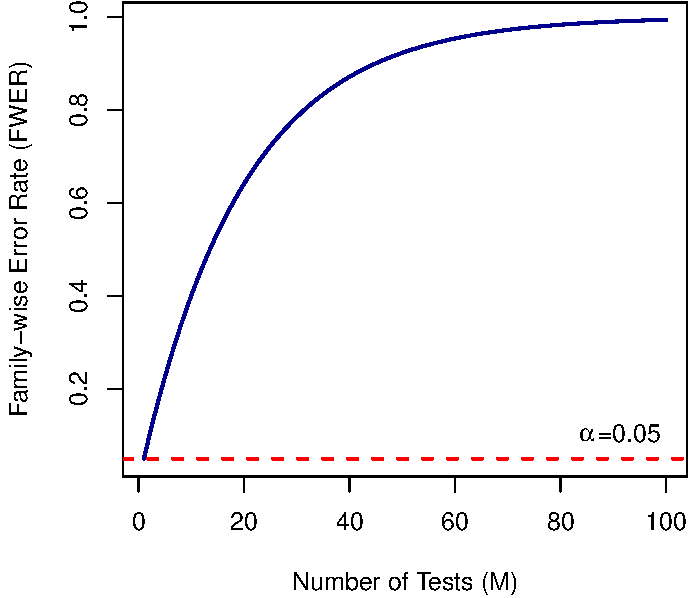
\includegraphics[width=0.5\textwidth]{FWER.pdf}
                  \caption{Family-Wise Error Rate Versus the Number of Hypothesis Tests, $M$.}\label{fig:FWER}
            \end{figure}
      \item A common value of $ M $ is $ \binom{m}{2} $: the number of pairwise comparisons necessary to compare each condition
            to every other condition.
            \begin{Example}{}{}
                  If $ m=5 $ and $ \alpha=0.05 $, then $ M=\binom{5}{2}=10 $. Therefore, $ \FWER=1-(1-0.05)^{10}=0.4013 $.
            \end{Example}
      \item Available to us are a variety of different statistical techniques that may be used to ensure the FWER
            does not exceed some threshold.
            \[ \FWER\le \alpha^\star \in[0,1] \]
            \begin{Remark}{General Notation}{}
                  \begin{itemize}
                        \item Denote the $ M $ null hypotheses as: $ \mathbf{H}_{0,1},\mathbf{H}_{0,2},\ldots,\mathbf{H}_{0,M} $.
                        \item Denote their corresponding $ p $-values as: $ p_1,p_2,\ldots,p_M $.
                  \end{itemize}
            \end{Remark}
            \begin{Example}{}{}
                  Suppose we test $ M =4 $ hypotheses, and the resulting $ p $-values are $ p_1 =0.015$, $ p_2=0.029 $,
                  $ p_3=0.008 $, and $ p_4=0.026 $.
            \end{Example}
\end{itemize}
\subsubsection*{The Bonferroni Correction}
\begin{itemize}
      \item This is the simplest method.
      \item Reject $ \mathbf{H}_{0,k} $ if
            \[ p_k\le \frac{\alpha^\star}{M} \quad\text{for }k=1,2,\ldots,M \]
            So, we test all $ M $ hypotheses at a significance level of $ \alpha^\star/M $.
      \item The procedure ensures $ \FWER\le \alpha^\star $. From Boole's Inequality,
            we know that
            \[ \FWER\le M\biggl(\frac{\alpha^\star}{M}\biggr)=\alpha^\star \]
      \item If we assume independence, the Bonferroni-corrected FWER becomes
            \[ 1-\biggl(1-\frac{\alpha^\star}{M} \biggr)^{\! M} \]
            Taking the limit of $ M \to\infty $ yields,
            \[ \lim\limits_{{M} \to {\infty}}\Biggl[1-\biggl(1-\frac{\alpha^\star}{M} \biggr)^{\! M}\Biggr]=1-e^{-\alpha^\star}  \]
            which for typical values of $ \alpha^\star $ in the range of $ \interval[open left]{0}{0.1} $ is approximately equal to $ \alpha^\star $.
            For example, if $ \alpha^\star=0.1 $, then the error is $ \approx 0.005 $. The asymptotic error rate
            and line of equality can be seen in~\Cref{fig:asymrate}.
            \begin{figure}[!htbp]
                  \centering
                  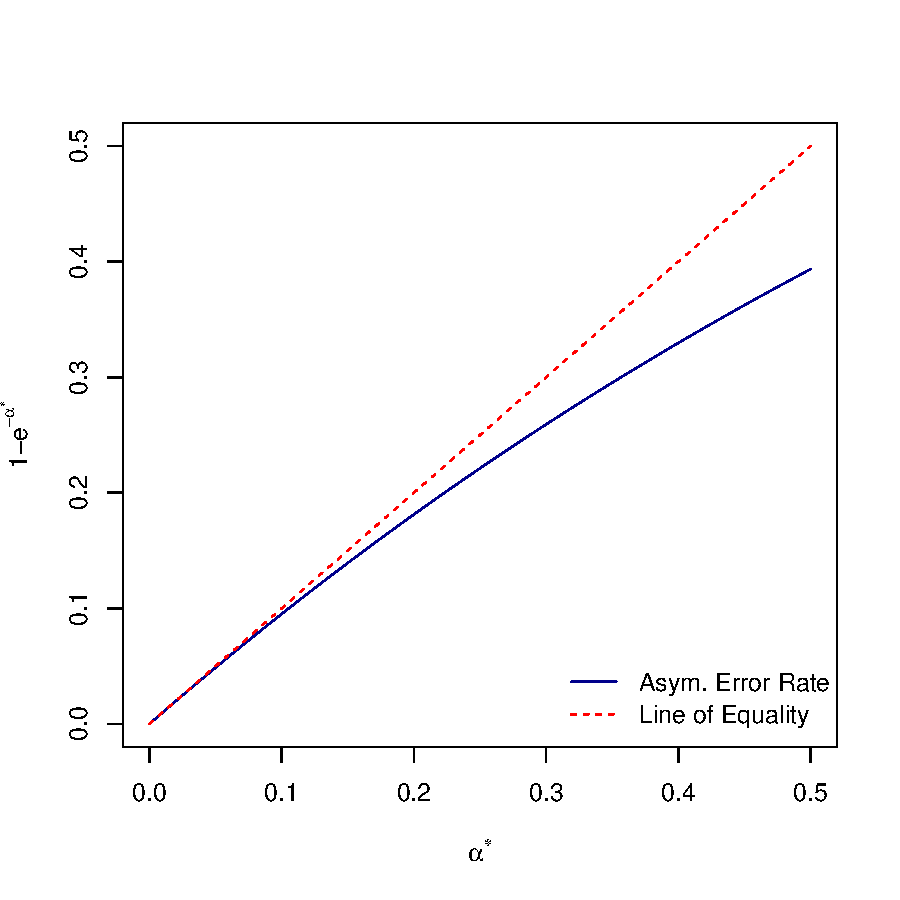
\includegraphics[width=0.5\textwidth]{asymrate.pdf}
                  \caption{Illustration of the Bonferroni Correction for Asymptotically Large $M$.}\label{fig:asymrate}
            \end{figure}
\end{itemize}
\begin{Example}{Four-test Example --- Bonferroni Correction}{}
      Let $ p_1=0.015 $, $ p_2=0.029 $, $ p_3=0.008 $, and $ p_4=0.026 $. Suppose that we wish to ensure
      $ \FWER\le \alpha^\star=0.05 $.

      \vspace{2mm}

      Under the Bonferroni Correction, we compare each
      $ p $-value to $ \alpha^\star/M=0.05/4=0.0125 $. Only $ p_3<0.0125 $, and hence
      only $ \mathbf{H}_{0,3} $ is rejected.
\end{Example}
\subsubsection*{The Šidák Correction}
\begin{itemize}
      \item This approach exploits the FWER formula derived when we assumed the $M$ tests were independent.
      \item Reject $ \mathbf{H}_{0,k} $ if
            \[ p_k\le 1-(1-\alpha^\star)^{1/M}\quad\text{for }k=1,2,\ldots,M \]
            \begin{Remark}{}{}
                  Where does the Šidák Correction come from?
                  \begin{align*}
                        \alpha^\star=\FWER=1-(1-\alpha)^M
                         & \iff 1-\alpha^\star = (1-\alpha)^M   \\
                         & \iff (1-\alpha^\star)^{1/M}=1-\alpha \\
                         & \iff \alpha=1-(1-\alpha^\star)^{1/M} \\
                  \end{align*}
            \end{Remark}
      \item This is actually not much different from the Bonferroni correction since
            \[ \frac{\alpha^\star}{M} \approx 1-(1-\alpha^\star)^{1/M} \]
            \begin{Example}{Bonferroni versus Šidák Correction}{}
                  Let $ \alpha^\star=0.05 $ and $ M=10 $. Then,
                  \[ \frac{\alpha^\star}{M} =0.005\quad\text{and}\quad 1-(1-\alpha^\star)^{1/M}=0.005116 \]
            \end{Example}
\end{itemize}
\begin{Example}{Four-test Example --- Šidák Correction}{}
      Let $ p_1=0.015 $, $ p_2=0.029 $, $ p_3=0.008 $, and $ p_4=0.026 $. Suppose that we wish to ensure
      $ \FWER\le \alpha^\star=0.05 $.

      \vspace{2mm}

      Under the Šidák Correction, we have
      \[ 1-(1-\alpha^\star)^{1/M}=1-(0.95)^{0.25}=0.012741 \]
      Therefore, we only reject $ \mathbf{H}_{0,3} $ since only $ p_3<0.012741 $.
\end{Example}
\subsubsection*{Holm's ``Step-Up'' Procedure}
\begin{itemize}
      \item The Bonferroni and Šidák corrections methods are very strict for large $M$.
            \begin{itemize}
                  \item In these cases \emph{most} null hypotheses will not be rejected.
                  \item If we're too strict, we basically stop rejecting null hypotheses thereby
                        eliminating Type I Errors, but we increase the Type II Errors.
            \end{itemize}
      \item Ideally we would have an approach that is less strict but still controls the FWER at some $ \alpha^\star $.
      \item This is exactly what Holm's Procedure gives us!
            \begin{framed}
                  \begin{enumerate}
                        \item Order the $M$ $p$-values from smallest to largest:
                              \[ p_{(1)},p_{(2)},\ldots,p_{(M)} \]
                              where $ p_{(k)} $ is the $ k^{\text{th}} $ smallest $ p $-value.
                        \item Starting from $ k=1 $ and continuing incrementally, compare
                              $ p_{(k)} $ to $ \alpha^\star/(M-k+1) $. Determine $ k^\star $,
                              the smallest value of $ k $ such that
                              \[ p_{(k)}>\frac{\alpha^\star}{M-k+1} \]
                        \item Reject the null hypotheses $ \mathbf{H}_{0,(1)},\ldots,\mathbf{H}_{0,(k^\star-1)} $
                              and do not reject $ \mathbf{H}_{0,(k^\star)},\ldots,\mathbf{H}_{0,(M)} $.
                  \end{enumerate}
            \end{framed}
      \item What's really happening?
            \begin{align*}
                  p_{(1)} & \text{ versus } \alpha^\star/M     \\
                  p_{(2)} & \text{ versus } \alpha^\star/(M-1) \\
                  p_{(3)} & \text{ versus } \alpha^\star/(M-2) \\
                          & \quad\;\vdots                      \\
                  p_{(M)} & \text{ versus } \alpha^\star
            \end{align*}
            We compare each $ p $-value to a Bonferroni-Corrected significance
            level based on the number of comparisons that remain to be
            made at a particular ``step.''
\end{itemize}
\begin{Theorem}{}{holm_FWER}
      Holm's procedure controls the family-wise error rate.
\end{Theorem}
\begin{Proof}{\Cref{thm:holm_FWER} \dagger}{}
      \begin{itemize}
            \item We need to show that $ \FWER=\Prob{V\ge 1}\le \alpha^\star\in[0,1] $ when using the Holm's procedure.
            \item Let $ p_{(1)},p_{(2)},\ldots,p_{(M)} $ be the ordered $ p $-values and let
                  $ \mathbf{H}_{0,(1)},\mathbf{H}_{0,(2)},\ldots,\mathbf{H}_{0,(M)} $ be the corresponding null hypotheses.
            \item Define $ K_0\subset \set{1,2,\ldots,M} $ to be the subset of indices which correspond
                  to true null hypotheses; that is, $ \mathbf{H}_{0,k} $ is true for $ k\in K_0 $.
            \item We can visualize the sequential decisions made in Holm's Procedure as follows:
                  \[ \overbracket{\underbracket{\mathbf{H}_{0,(1)}\cdots\mathbf{H}_{0,(h-1)}}_{\text{these are false $\mathbf{H}_0$'s}}\mathbf{H}_{0,(h)}\cdots \mathbf{H}_{0,(R)}}^{\text{these are rejected}}\mid \underbracket{\mathbf{H}_{0,(R+1)}\cdots\mathbf{H}_{0,(M)}}_{\text{these are not rejected}} \]
      \end{itemize}
      Let $ \mathbf{H}_{0,(h)} $ be the first \emph{true} $ \mathbf{H}_0 $ that was rejected. Since it was rejected by Holm's procedure, we know that
      \[ p_{(h)}\le \frac{\alpha^\star}{M-h+1} \]
      Also, clearly we must have $ h-1\le M-M_0 $ since $ M-M_0 $ is the total number of false $ \mathbf{H}_0 $'s and $ h-1 $ is the number of false
      $ \mathbf{H}_0 $'s encountered by test $ h $. And so,
      \[
            M_0\le M-h+1
            \iff \frac{1}{M_0} \ge \frac{1}{M-h+1}
            \iff \frac{\alpha^\star}{M_0} \ge \frac{\alpha^\star}{M-h+1}
      \]
      Thus, we must have $ p_{(h)}\le \alpha^\star/(M-h+1)\le \alpha^\star/M_0 $. Therefore,
      \begin{align*}
            \FWER
             & =\Prob*{V\ge 1}                                                                                                                    \\
             & =\Prob*{\text{At least one Type I Error in $M$ tests}}                                                                             \\
             & =\Prob*{\text{Reject at least one true $\mathbf{H}_0$}}                                                                            \\
             & =\Prob*{\exists\, k\in K_0\text{ such that }p_k\le \frac{\alpha^\star}{M_0}}                                                       \\
             & =\Prob*{\bigcup_{k\in K_0}p_k\le \frac{\alpha^\star}{M_0}}                                                                         \\
             & \le \sum_{k\in K_0}\Prob*{p_k\le \frac{\alpha^\star}{M_0}}                   &  & \text{by Boole's Inequality}                     \\
             & =\sum_{k\in K_0}\frac{\alpha^\star}{M_0}                                     &  & \!\!\!\!\begin{tabular}{l}
                  \text{since $p$-values for true null} \\
                  \text{hypotheses follow a $\uniform{0,1}$ distribution}
            \end{tabular}               \\
             & =M_0\biggl(\frac{\alpha^\star}{M_0}\biggr)                                   &  & \text{since the set $K_0$ has cardinality $M_0$} \\
             & =\alpha^\star
      \end{align*}
      Therefore, $ \FWER\le \alpha^\star $ as required.
\end{Proof}
\begin{Example}{Four-test Example ($ M=4 $) --- Holm's Procedure}{}
      Let $ p_1=0.015 $, $ p_2=0.029 $, $ p_3=0.008 $, and $ p_4=0.026 $. Suppose that we wish to ensure
      $ \FWER\le \alpha^\star=0.05 $.
      \begin{align*}
            p_{(1)}=p_3=0.008 & \text{ versus } \alpha^\star/M=0.05/4=0.0125     \\
            p_{(2)}=p_1=0.015 & \text{ versus } \alpha^\star/(M-1)=0.05/3=0.0167 \\
            p_{(3)}=p_4=0.026 & \text{ versus } \alpha^\star/(M-2)=0.05/2=0.025  \\
            p_{(4)}=p_2=0.029 & \text{ versus } \alpha^\star/(M-3)=0.05/1=0.05
      \end{align*}
      We reject $ \mathbf{H}_{0,(1)}=\mathbf{H}_{0,3} $ and $ \mathbf{H}_{0,(2)}=\mathbf{H}_{0,1} $. We do not reject
      $ \mathbf{H}_{0,(3)}=\mathbf{H}_{0,4} $ or $ \mathbf{H}_{0,(4)}=\mathbf{H}_{0,2} $. Note that $ k^\star=3 $.
\end{Example}
\begin{itemize}
      \item The decision process for all three of these methods can be visualized by plotting the ordered $p$-values
            $ p_{(k)} $ versus their ranks $ k=1,2,\ldots,M $ and overlay the significance thresholds which can
            be seen in~\Cref{fig:pvsrank1}.
            \begin{figure}[!htbp]
                  \centering
                  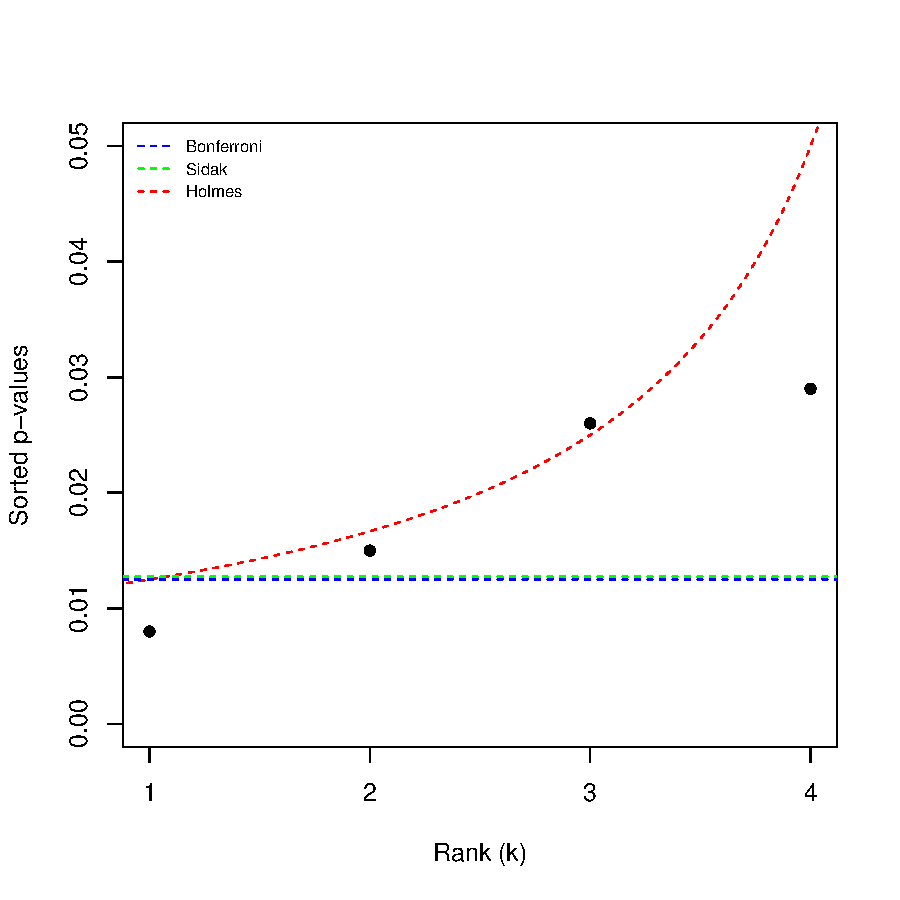
\includegraphics[width=0.5\textwidth]{pvsrank1.pdf}
                  \caption{Significance Thresholds for Several Methods of Correction (1).}\label{fig:pvsrank1}
            \end{figure}
      \item The Bonferroni correction is most strict, followed by the Šidák correction, then by Holm's procedure.
\end{itemize}
\subsubsection*{Adjusted $ p $-values}
\begin{itemize}
      \item So far we have framed each of the correction procedures above as an adjustment to the significance
            threshold against which each $p$-value is compared.
      \item Alternatively (and equivalently) we could invert this process and frame the decision in terms of a
            comparison of \emph{adjusted $p$-values} to $ \alpha^\star $.
      \item This is more familiar (compare our $ p $-values to some constant threshold $ \alpha^\star $).
            \begin{itemize}
                  \item We just need to adjust our $p$-values first.
            \end{itemize}
      \item The decisions made with the following adjusted $p$-values are identical to that achieved by comparing
            unadjusted $p$-values to the methods' adjusted significance thresholds.
            \begin{itemize}
                  \item Bonferroni: Reject $ \mathbf{H}_{0,k} $ if $ p_k^\star\le \alpha^\star $ where
                        \[ p_k^\star=Mp_k \]
                        \begin{Example}{Bonferroni's Adjusted $ p $-values}{}
                              In our four-test example, $ p_1^\star=0.06 $, $ p_2^\star=0.116 $, $ p_3^\star=0.032 $, and $ p_4^\star=0.104 $.
                              Comparing to $ \alpha^\star=0.05 $, we reject $ \mathbf{H}_{0,3} $.
                        \end{Example}
                  \item Šidák: Reject $ \mathbf{H}_{0,k} $ if $ p_k^\star\le \alpha^\star $ where
                        \[ p_k^\star=1-(1-p_k)^M \]
                        \begin{Example}{Šidák's Adjusted $ p $-values}{}
                              In our four-test example, $ p_1^\star=0.0587 $, $ p_2^\star=0.111 $, $ p_3^\star=0.0316 $, and $ p_4^\star=0.1 $.
                              Comparing to $ \alpha^\star=0.05 $, we reject $ \mathbf{H}_{0,3} $.
                        \end{Example}
                  \item Holm: Reject $ \mathbf{H}_{0,k} $ if $ p_{(k)}^\star\le \alpha^\star $ where
                        \[ p_{(k)}^\star=\max_{j\le k}\set*{p_{(j)}(M-j+1)} \]
                        \begin{Example}{Holm's Adjusted $ p $-values}{}
                              Let $ p_1=0.015 $, $ p_2=0.029 $, $ p_3=0.008 $, and $ p_4=0.026 $.
                              \[ \begin{array}{ccccl}
                                          k & p_{(k)} & M-k+1 & p_{(k)}(M-k+1) & p_{(k)}^\star=\max_{j\le k}\set*{p_{(j)}(M-j+1)}      \\
                                          \midrule
                                          1 & 0.008   & 4     & 0.032          & \max\set{0.032}=0.032=p_{(1)}^\star                   \\
                                          2 & 0.015   & 3     & 0.045          & \max\set{0.032,0.045}=0.045=p_{(2)}^\star             \\
                                          3 & 0.026   & 2     & 0.052          & \max\set{0.032,0.045,0.052}=0.052=p_{(3)}^\star       \\
                                          4 & 0.029   & 1     & 0.029          & \max\set{0.032,0.045,0.052,0.029}=0.052=p_{(4)}^\star
                                    \end{array} \]
                              Thus, $ p_1^\star=p_{(2)}^\star=0.045 $, $ p_2^\star=p_{(4)}^\star=0.052 $, $ p_3^\star=p_{(1)}^\star=0.032 $, and
                              $ p_4^\star=p_{(3)}^\star=0.052 $. Comparing to $ \alpha^\star=0.05 $, we reject
                              $ \mathbf{H}_{0,1} $ and $ \mathbf{H}_{0,3} $.
                        \end{Example}
            \end{itemize}
      \item Implemented in R with \code{p.adjust()}.
\end{itemize}
\subsection{False Discovery Rate}
\begin{itemize}
      \item In the mid-1900s, Statisticians developed FWER methods with $ M\approx 20 $ comparisons in mind.
      \item In the era of Big Data, much larger values of $M$ are typical.
      \item For larger values of $M$, traditional methods tend to be very conservative, and so FWER is perhaps
            not the best metric to control.
      \item More recently, emphasis has been placed on controlling the \emph{rate} at which Type I Errors occur.
            \begin{Definition}{False discovery proportion}{}
                  The \textbf{false discovery proportion} (FDP) is
                  \[ Q=\frac{V}{R} \]
                  Thus, $ Q $ is the proportion of all rejected null hypotheses that were rejected
                  in error.
            \end{Definition}
      \item In particular, interest lies in controlling the \textbf{false discovery rate} (FDR).
            \begin{Definition}{False discovery rate}{}
                  The \textbf{false discovery rate} is
                  \[ \E{Q}=\E*{\frac{V}{R}} \]
            \end{Definition}
      \item Unlike the FWER, the FDR is adaptive in the sense that the number of Type I Errors $V$ has different
            implications depending on the size of $M$. That is,
            \begin{itemize}
                  \item Two Type I Errors in 10 tests might be unacceptable.
                  \item Two Type I Errors in 100 tests might be okay.
            \end{itemize}
      \item Methods that control the FDR are less strict than methods that control FWER\@.
            \begin{itemize}
                  \item More Type I Errors will occur with such methods, but this is viewed as acceptable when $M$ is
                        very large.
            \end{itemize}
\end{itemize}
\subsubsection*{Benjamini-Hochberg Procedure}
\begin{itemize}
      \item The Benjamini-Hochberg (BH) procedure for controlling FDR is a sequentially rejective procedure
            much like Holm's procedure for controlling FWER\@. The main difference is the threshold we
            compare the ordered $ p $-values to.
      \item We summarize the BH procedure, which aims to ensure $ \text{FDR}\le \alpha^\star $:
            \begin{framed}
                  \begin{enumerate}
                        \item Order the $M$ $p$-values from smallest to largest:
                              \[ p_{(1)},p_{(2)},\ldots,p_{(M)} \]
                              where $ p_{(k)} $ is the $ k^{\text{th}} $ smallest $ p $-value.
                        \item Starting from $ k=1 $ and continuing incrementally, compare
                              $ p_{(k)} $ to $ k\alpha^\star/M $. Determine $ k^\star $
                              the largest value of $ k $ such that
                              \[ p_{(k)}\le \frac{k\alpha^\star}{M}  \]
                        \item Reject the null hypotheses $ \mathbf{H}_{0,(1)},\ldots,\mathbf{H}_{0,(k^\star)} $
                              and do not reject $ \mathbf{H}_{0,(k^\star+1)},\ldots,\mathbf{H}_{0,(M)} $.
                  \end{enumerate}
            \end{framed}
      \item The decision process associated with this procedure is best visualized with a plot of the ordered $p$-values
            $ p_{(k)} $ versus their ranks $ k=1,2,\ldots,M $ with the significance threshold overlaid which can
            be seen in~\Cref{fig:pvsrank2}.
            \begin{itemize}
                  \item The BH significance threshold is the line with intercept $0$ and slope $ \alpha^\star/M $.
            \end{itemize}
            \begin{figure}[!htbp]
                  \centering
                  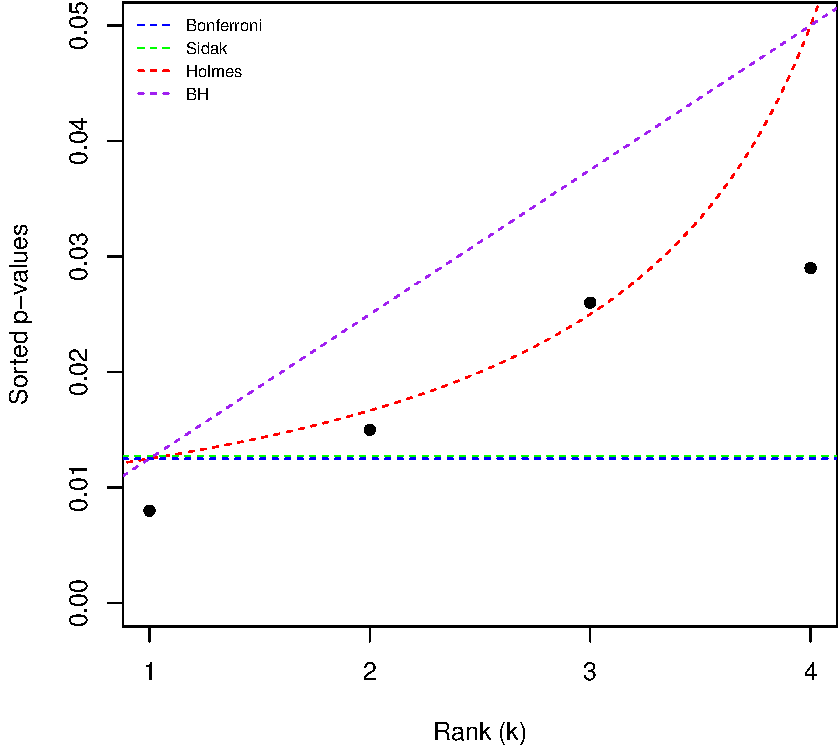
\includegraphics[width=0.5\textwidth]{pvsrank2.pdf}
                  \caption{Significance Thresholds for Several Methods of Correction (2).}\label{fig:pvsrank2}
            \end{figure}
            \begin{Example}{Four-test Example --- Benjamini-Hochberg Procedure}{}
                  Let $ p_1=0.015 $, $ p_2=0.029 $, $ p_3=0.008 $, and $ p_4=0.026 $. Suppose that we wish to ensure
                  $ \FWER\le \alpha^\star=0.05 $. Since all $ p $-values fall below the purple line in~\Cref{fig:pvsrank2},
                  we reject all four null hypotheses.
            \end{Example}
      \item This threshold is much less strict than any of the FWER-control thresholds, but this is the appeal of
            the approach.
      \item The procedure that guarantees $ \text{FDR}\le \alpha^\star $ is beyond the scope of this course.
            However, the proof can be found in~\citet{benjamini} and~\citet{storey}.
      \item Like the FWER controlling methods we can define Benjamini-Hochberg-adjusted $p$-values and invert
            the decision framework by comparing the adjusted $ p $-values to $ \alpha^\star $.
            \begin{itemize}
                  \item Reject $ \mathbf{H}_{0,(k)} $ if $ p_{(k)}^\star\le \alpha^\star $ where
                        \[ p_{(k)}^\star=\min_{j\ge k}\set*{\frac{Mp_{(j)}}{j}} \]
                        \begin{Example}{Benjamini-Hochberg Procedure's Adjusted $ p $-values}{}
                              Let $ p_1=0.015 $, $ p_2=0.029 $, $ p_3=0.008 $, and $ p_4=0.026 $.
                              \[ \begin{array}{cccl}
                                          k & p_{(k)} & M p_{(k)}/k & p_{(k)}^\star=\min_{j\ge k}\set*{Mp_{(j)}/j}          \\
                                          \midrule
                                          1 & 0.008   & 0.032       & \min\set{0.032,0.030,0.035,0.029}=0.029=p_{(1)}^\star \\
                                          2 & 0.015   & 0.030       & \min\set{0.030,0.035,0.029}=0.029=p_{(2)}^\star       \\
                                          3 & 0.026   & 0.035       & \min\set{0.035,0.029}=0.029=p_{(3)}^\star             \\
                                          4 & 0.029   & 0.029       & \min\set{0.029}=0.029=p_{(4)}^\star
                                    \end{array} \]
                              Thus, $ p_1^\star=p_{(2)}^\star=0.029 $, $ p_2^\star=p_{(4)}^\star=0.029 $, $ p_3^\star=p_{(1)}^\star=0.029 $,
                              and $ p_4^\star=p_{(3)}^\star=0.029 $. Comparing to $ \alpha^\star=0.05 $,
                              we reject all $ \mathbf{H}_{0} $'s.
                        \end{Example}
            \end{itemize}
\end{itemize}
\href{https://github.com/Hextical/university-notes/blob/master/year-3/semester-3/STAT 430/code/W4/Multiple_testing_example.R}{[R Code] \texttt{Multiple\_testing\_example}}
\subsection{Sample Size Determination}
\begin{itemize}
      \item So what does all of this mean for power analyses and sample size calculations?
      \item There is a duality between significance level and power.
            \begin{itemize}
                  \item All else equal, reducing a test's significance level will increase the Type II Error rate and hence
                        decrease power.
                  \item Play around with \href{https://nathaniel-t-stevens.shinyapps.io/ErrorIllustrator/}{this interactive app} to gain comfort with this notion.
                        \begin{itemize}
                              \item Assume $ \mathcal{R}=\set*{t\mid t\ge z_\alpha} $.
                              \item Recall that: \begin{itemize}
                                          \item $ \alpha=\Prob*{\text{Type I Error}}=\Prob*{T\in\mathcal{R}\given \text{$ \mathbf{H}_0 $ is true}}=\Prob*{T\ge z_\alpha\given \text{$ \mathbf{H}_0 $ is true}}$.
                                          \item $ \beta=\Prob*{\text{Type II Error}}=\Prob*{T\notin\mathcal{R}\given \text{$ \mathbf{H}_\text{A} $ is true}}=\Prob*{T< z_\alpha\given \text{$ \mathbf{H}_\text{A} $ is true}} $.
                                    \end{itemize}
                        \end{itemize}
            \end{itemize}
      \item Thus, all the correction procedures discussed (which decrease the effective significance level)
            negatively impact power.
      \item In order to maintain power at some pre-specified level, we must compensate by increasing the sample
            size.
      \item Therefore, the more complicated your experiment (i.e., the more conditions it has), the larger your
            sample sizes will need to be.
            \begin{itemize}
                  \item Such modifications can be accounted for when selecting a sample size.
                  \item The significance level you use in your sample size calculations should be the adjusted one based
                        on the correction method you use.
                  \item This is easier to do with \emph{some} correction methods than others.
            \end{itemize}
\end{itemize}


\subsection*{Example: Homelessness and Physical Health}
Data Source: Kleinman, K and Horton, NJ. SAS and R: \emph{Data
      Management, Statistical Analysis, and Graphics}. CRC Press.

The HELP (Health Evaluation and Linkage to Primary Care) study
was a clinical trial for adult patients recruited from a detoxification
unit. Patients with no primary care physician were randomized to
receive a multidisciplinary assessment and a brief motivational
intervention or usual care, with the goal of linking them to primary
medical care.

\textbf{Secondary Analysis}: Does homelessness affect physical health?
\url{http://sas-and-r.blogspot.com/2010/04/example-734-propensity-scores-and.html}

Available data:
\begin{itemize}
      \item \texttt{pcs}: measure of physical health via 36 question questionnaire
            (mean $48.05$, range $[14.07, 74.81]$).
      \item \texttt{homeless}: binary indicator of homelessness ($46.14\%$ homeless).
      \item \texttt{age}: in years (mean $35.65$, range $[19.00, 60.00]$).
      \item \texttt{female}: indicator of female sex ($23.62\%$ female).
      \item \texttt{i1}: alcohol intake per day (mean $17.9$, median $13.0$, range $[0,142]$).
      \item \texttt{mcs}: mental component summary measure
            (mean $31.68$, range $[6.76, 62.18]$).
\end{itemize}
\begin{itemize}
      \item Linear model for the association between homelessness and
            physical health:
            %\begin{noindent}
\begin{knitrout}
\definecolor{shadecolor}{rgb}{0.969, 0.969, 0.969}\color{fgcolor}\begin{kframe}
\begin{alltt}
\hlstd{ds} \hlkwb{<-} \hlkwd{read.csv}\hlstd{(}\hlstr{"data/help.csv"}\hlstd{)}
\hlkwd{attach}\hlstd{(ds)}
\hlkwd{summary}\hlstd{(}\hlkwd{lm}\hlstd{(pcs} \hlopt{~} \hlstd{homeless))}
\end{alltt}
\begin{verbatim}

Call:
lm(formula = pcs ~ homeless)

Residuals:
    Min      1Q  Median      3Q     Max 
-34.927  -7.903   0.644   8.387  25.805 

Coefficients:
            Estimate Std. Error t value Pr(>|t|)    
(Intercept)   49.001      0.688  71.220   <2e-16 ***
homeless      -2.064      1.013  -2.038   0.0422 *  
---
Signif. codes:  0 '***' 0.001 '**' 0.01 '*' 0.05 '.' 0.1 ' ' 1

Residual standard error: 10.75 on 451 degrees of freedom
Multiple R-squared:  0.009123,	Adjusted R-squared:  0.006926 
F-statistic: 4.152 on 1 and 451 DF,  p-value: 0.04216
\end{verbatim}
\end{kframe}
\end{knitrout}
      %\end{noindent}
            Unadjusted analysis: significant association between homelessness
            and physical health.
\end{itemize}
\subsection{Estimation}
\begin{itemize}
      \item Fit a logistic model for the propensity score
            %\begin{noindent}
\begin{knitrout}
\definecolor{shadecolor}{rgb}{0.969, 0.969, 0.969}\color{fgcolor}\begin{kframe}
\begin{alltt}
\hlstd{glm1} \hlkwb{<-} \hlkwd{glm}\hlstd{(homeless} \hlopt{~} \hlstd{age} \hlopt{+} \hlkwd{factor}\hlstd{(female)} \hlopt{+} \hlstd{i1} \hlopt{+} \hlstd{mcs,} \hlkwc{family} \hlstd{= binomial)}
\hlstd{PS} \hlkwb{<-} \hlstd{glm1}\hlopt{$}\hlstd{fitted.values}
\hlkwd{summary}\hlstd{(glm1)}
\end{alltt}
\begin{verbatim}

Call:
glm(formula = homeless ~ age + factor(female) + i1 + mcs, family = binomial)

Deviance Residuals: 
    Min       1Q   Median       3Q      Max  
-1.7603  -1.0271  -0.8211   1.2039   1.6332  

Coefficients:
                 Estimate Std. Error z value Pr(>|z|)    
(Intercept)     -0.658259   0.518953  -1.268   0.2046    
age              0.013659   0.012965   1.054   0.2921    
factor(female)1 -0.454530   0.237011  -1.918   0.0551 .  
i1               0.024878   0.005782   4.303 1.68e-05 ***
mcs             -0.009983   0.007768  -1.285   0.1987    
---
Signif. codes:  0 '***' 0.001 '**' 0.01 '*' 0.05 '.' 0.1 ' ' 1

(Dispersion parameter for binomial family taken to be 1)

    Null deviance: 625.28  on 452  degrees of freedom
Residual deviance: 592.54  on 448  degrees of freedom
AIC: 602.54

Number of Fisher Scoring iterations: 4
\end{verbatim}
\end{kframe}
\end{knitrout}
      %\end{noindent}
      \item Which variables should be included in the PS model? Real
            confounders and variables that are predictive of the outcome.
            %\begin{noindent}
\begin{knitrout}
\definecolor{shadecolor}{rgb}{0.969, 0.969, 0.969}\color{fgcolor}\begin{kframe}
\begin{alltt}
\hlkwd{summary}\hlstd{(}\hlkwd{lm}\hlstd{(pcs} \hlopt{~} \hlstd{age))}\hlopt{$}\hlstd{coef}
\end{alltt}
\begin{verbatim}
              Estimate Std. Error   t value     Pr(>|t|)
(Intercept) 59.4549837 2.33874676 25.421728 4.125943e-89
age         -0.3199256 0.06411778 -4.989655 8.651612e-07
\end{verbatim}
\begin{alltt}
\hlkwd{summary}\hlstd{(}\hlkwd{lm}\hlstd{(pcs} \hlopt{~} \hlstd{female))}\hlopt{$}\hlstd{coef}
\end{alltt}
\begin{verbatim}
             Estimate Std. Error   t value      Pr(>|t|)
(Intercept) 48.986239  0.5732719 85.450274 1.076730e-280
female      -3.969879  1.1795541 -3.365576  8.291456e-04
\end{verbatim}
\begin{alltt}
\hlkwd{summary}\hlstd{(}\hlkwd{lm}\hlstd{(pcs} \hlopt{~} \hlstd{i1))}\hlopt{$}\hlstd{coef}
\end{alltt}
\begin{verbatim}
              Estimate Std. Error   t value      Pr(>|t|)
(Intercept) 49.9424609 0.66766179 74.802036 2.407295e-256
i1          -0.1057625 0.02487199 -4.252273  2.573816e-05
\end{verbatim}
\begin{alltt}
\hlkwd{summary}\hlstd{(}\hlkwd{lm}\hlstd{(pcs} \hlopt{~} \hlstd{mcs))}\hlopt{$}\hlstd{coef}
\end{alltt}
\begin{verbatim}
               Estimate Std. Error   t value      Pr(>|t|)
(Intercept) 45.10957488 1.34341383 33.578317 9.114672e-125
mcs          0.09278014 0.03931041  2.360192  1.869034e-02
\end{verbatim}
\end{kframe}
\end{knitrout}
      %\end{noindent}
      \item Check that there is a reasonable amount of overlap in the
            propensity scores between the two groups:
            %\begin{noindent}
\begin{knitrout}
\definecolor{shadecolor}{rgb}{0.969, 0.969, 0.969}\color{fgcolor}\begin{kframe}
\begin{alltt}
\hlkwd{summary}\hlstd{(PS[homeless} \hlopt{==} \hlnum{0}\hlstd{])}
\end{alltt}
\begin{verbatim}
   Min. 1st Qu.  Median    Mean 3rd Qu.    Max. 
 0.2137  0.3474  0.4040  0.4297  0.4980  0.7876 
\end{verbatim}
\begin{alltt}
\hlkwd{summary}\hlstd{(PS[homeless} \hlopt{==} \hlnum{1}\hlstd{])}
\end{alltt}
\begin{verbatim}
   Min. 1st Qu.  Median    Mean 3rd Qu.    Max. 
 0.2635  0.4003  0.4739  0.4984  0.5768  0.9643 
\end{verbatim}
\end{kframe}
\end{knitrout}
      %\end{noindent}
            \begin{itemize}
                  \item Mean propensity to homelessness is larger in the homeless
                        group.
                  \item There are no non-homeless subjects with a propensity score
                        $> 0.8$.
            \end{itemize}
            %\begin{noindent}
\begin{knitrout}
\definecolor{shadecolor}{rgb}{0.969, 0.969, 0.969}\color{fgcolor}

{\centering 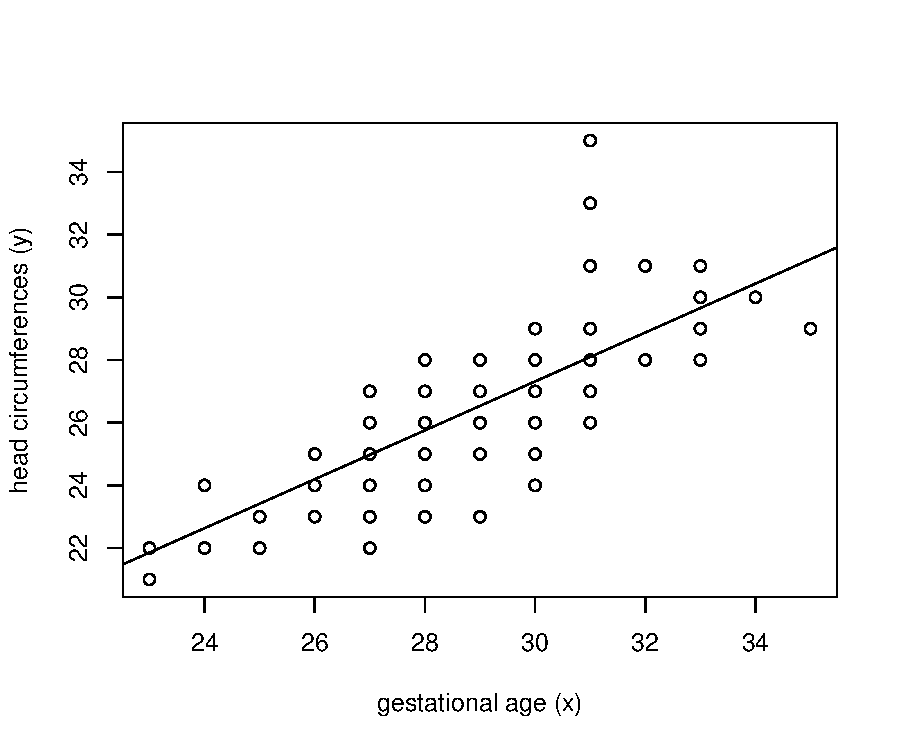
\includegraphics[width=\maxwidth]{figure/unnamed-chunk-8-1} 

}


\end{knitrout}
      %\end{noindent}
\end{itemize}
\subsection{Matching}
In R, the \texttt{Matching} library provides tools for matching and analysis.
%\begin{noindent}
\begin{knitrout}
\definecolor{shadecolor}{rgb}{0.969, 0.969, 0.969}\color{fgcolor}\begin{kframe}
\begin{alltt}
\hlkwd{library}\hlstd{(Matching)}
\hlstd{rr} \hlkwb{<-} \hlkwd{Match}\hlstd{(}\hlkwc{Y} \hlstd{= pcs,} \hlkwc{Tr} \hlstd{= homeless,} \hlkwc{X} \hlstd{= PS,} \hlkwc{M} \hlstd{=} \hlnum{1}\hlstd{,} \hlkwc{replace} \hlstd{=} \hlnum{TRUE}\hlstd{,}
  \hlkwc{estimand} \hlstd{=} \hlstr{"ATE"}\hlstd{)}
\hlkwd{summary}\hlstd{(rr)}
\end{alltt}
\begin{verbatim}

Estimate...  -1.2774 
AI SE......  1.2311 
T-stat.....  -1.0376 
p.val......  0.29945 

Original number of observations..............  453 
Original number of treated obs...............  209 
Matched number of observations...............  453 
Matched number of observations  (unweighted).  536 
\end{verbatim}
\begin{alltt}
\hlcom{# average causal effect estimate}
\hlstd{rr}\hlopt{$}\hlstd{est}
\end{alltt}
\begin{verbatim}
          [,1]
[1,] -1.277365
\end{verbatim}
\begin{alltt}
\hlcom{# standard error of ACE estimate}
\hlstd{rr}\hlopt{$}\hlstd{se}
\end{alltt}
\begin{verbatim}
[1] 1.231057
\end{verbatim}
\begin{alltt}
\hlcom{# p-value for testing ACE=0}
\hlkwd{pnorm}\hlstd{(rr}\hlopt{$}\hlstd{est}\hlopt{/}\hlstd{rr}\hlopt{$}\hlstd{se)} \hlopt{*} \hlnum{2}
\end{alltt}
\begin{verbatim}
          [,1]
[1,] 0.2994486
\end{verbatim}
\end{kframe}
\end{knitrout}
%\end{noindent}
\begin{itemize}
      \item The causal estimate of $-1.28$ in the matched comparison is
            not statistically significant ($p=0.30$).
      \item Note that the specific results depend on the particular options
            that are selected for the matching.
\end{itemize}
\subsection{Stratification}
We will stratify the dataset into four ($K=4$) approximately equally
sized groups.
%\begin{noindent}
\begin{knitrout}
\definecolor{shadecolor}{rgb}{0.969, 0.969, 0.969}\color{fgcolor}\begin{kframe}
\begin{alltt}
\hlstd{breakvals} \hlkwb{<-} \hlkwd{fivenum}\hlstd{(PS)}
\hlstd{strata} \hlkwb{<-} \hlkwd{cut}\hlstd{(PS,} \hlkwc{breaks} \hlstd{= breakvals,} \hlkwc{labels} \hlstd{=} \hlkwd{c}\hlstd{(}\hlstr{"bot quart"}\hlstd{,}
  \hlstr{"2nd quart"}\hlstd{,} \hlstr{"3rd quart"}\hlstd{,} \hlstr{"top quart"}\hlstd{),} \hlkwc{include.lowest} \hlstd{=} \hlnum{TRUE}\hlstd{)}
\hlstd{strata[}\hlnum{1}\hlopt{:}\hlnum{5}\hlstd{]}
\end{alltt}
\begin{verbatim}
[1] 3rd quart top quart 2nd quart bot quart 3rd quart
Levels: bot quart 2nd quart 3rd quart top quart
\end{verbatim}
\begin{alltt}
\hlkwd{table}\hlstd{(strata)}
\end{alltt}
\begin{verbatim}
strata
bot quart 2nd quart 3rd quart top quart 
      114       113       113       113 
\end{verbatim}
\end{kframe}
\end{knitrout}
%\end{noindent}
Boxplots of the PCS scores for homeless and non-homeless by the
four strata of propensity scores (\url{http://sas-and-r.blogspot.com/search?q=7.36}):
%\begin{noindent}
\begin{knitrout}
\definecolor{shadecolor}{rgb}{0.969, 0.969, 0.969}\color{fgcolor}

{\centering 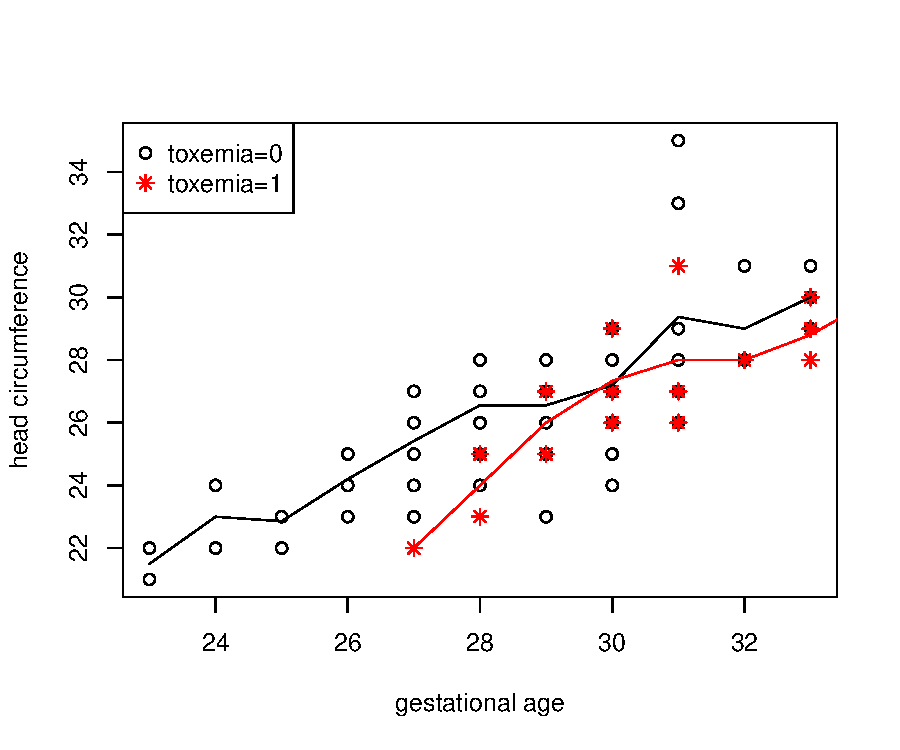
\includegraphics[width=\maxwidth]{figure/unnamed-chunk-11-1} 

}


\end{knitrout}
%\end{noindent}
\begin{itemize}
      \item The difference between the median PCS scores is smaller
            within each of the quartiles of the propensity scores than the
            difference between medians overall.
      \item Proportion of subjects in the two groups varies by strata.
      \item Use a $t$-test in each stratum to test whether difference in mean
            PCS is significant between homeless and non-homeless
            subjects.
      \item Mean \texttt{pcs} is lower in 3 out of 4 strata but not statistically
            significant.
      \item Little credible evidence for a health cost ascribable to
            homelessness.
\end{itemize}
%\begin{noindent}
\begin{knitrout}
\definecolor{shadecolor}{rgb}{0.969, 0.969, 0.969}\color{fgcolor}\begin{kframe}
\begin{alltt}
\hlstd{stratdf} \hlkwb{<-} \hlkwd{data.frame}\hlstd{(pcs, homeless, strata)}
\hlstd{out} \hlkwb{<-} \hlkwd{by}\hlstd{(stratdf, strata,} \hlkwa{function}\hlstd{(}\hlkwc{mydataframe}\hlstd{) \{}
  \hlkwd{with}\hlstd{(mydataframe,} \hlkwd{t.test}\hlstd{(pcs[homeless} \hlopt{==} \hlnum{0}\hlstd{], pcs[homeless} \hlopt{==}
    \hlnum{1}\hlstd{]))}
\hlstd{\})}
\hlcom{# bot quart: t = 0.80603, df = 58.564, p-value = 0.4235}

\hlcom{# 2nd quart: t = -0.10106, df = 101.08, p-value = 0.9197}

\hlcom{# 3rd quart: t = 0.82302, df = 110.92, p-value = 0.4123}

\hlcom{# top quart: t = 0.92219, df = 74.798, p-value = 0.3594}

\hlkwd{lm}\hlstd{(pcs} \hlopt{~} \hlstd{homeless,} \hlkwc{data} \hlstd{= ds[strata} \hlopt{==} \hlstr{"bot quart"}\hlstd{, ])}\hlopt{$}\hlstd{coef}
\end{alltt}
\begin{verbatim}
(Intercept)    homeless 
   49.88714    -1.79067 
\end{verbatim}
\begin{alltt}
\hlkwd{lm}\hlstd{(pcs} \hlopt{~} \hlstd{homeless,} \hlkwc{data} \hlstd{= ds[strata} \hlopt{==} \hlstr{"2nd quart"}\hlstd{, ])}\hlopt{$}\hlstd{coef}
\end{alltt}
\begin{verbatim}
(Intercept)    homeless 
 49.3708866   0.2041892 
\end{verbatim}
\begin{alltt}
\hlkwd{lm}\hlstd{(pcs} \hlopt{~} \hlstd{homeless,} \hlkwc{data} \hlstd{= ds[strata} \hlopt{==} \hlstr{"3rd quart"}\hlstd{, ])}\hlopt{$}\hlstd{coef}
\end{alltt}
\begin{verbatim}
(Intercept)    homeless 
   49.44396    -1.67437 
\end{verbatim}
\begin{alltt}
\hlkwd{lm}\hlstd{(pcs} \hlopt{~} \hlstd{homeless,} \hlkwc{data} \hlstd{= ds[strata} \hlopt{==} \hlstr{"top quart"}\hlstd{, ])}\hlopt{$}\hlstd{coef}
\end{alltt}
\begin{verbatim}
(Intercept)    homeless 
  46.075841   -1.985963 
\end{verbatim}
\end{kframe}
\end{knitrout}
%\end{noindent}
\subsection{Inverse Probability Weighting}
%\begin{noindent}
\begin{knitrout}
\definecolor{shadecolor}{rgb}{0.969, 0.969, 0.969}\color{fgcolor}\begin{kframe}
\begin{alltt}
\hlstd{ACE.1} \hlkwb{<-} \hlnum{1}\hlopt{/}\hlkwd{length}\hlstd{(PS)} \hlopt{*} \hlstd{(}\hlkwd{sum}\hlstd{(homeless} \hlopt{*} \hlstd{pcs}\hlopt{/}\hlstd{PS)} \hlopt{-} \hlkwd{sum}\hlstd{((}\hlnum{1} \hlopt{-} \hlstd{homeless)} \hlopt{*}
  \hlstd{pcs}\hlopt{/}\hlstd{(}\hlnum{1} \hlopt{-} \hlstd{PS)))}
\hlstd{ACE.1}
\end{alltt}
\begin{verbatim}
[1] -1.652115
\end{verbatim}
\begin{alltt}
\hlstd{ACE.2} \hlkwb{<-} \hlkwd{sum}\hlstd{(homeless} \hlopt{*} \hlstd{pcs}\hlopt{/}\hlstd{PS)}\hlopt{/}\hlkwd{sum}\hlstd{(homeless}\hlopt{/}\hlstd{PS)} \hlopt{-} \hlkwd{sum}\hlstd{((}\hlnum{1} \hlopt{-} \hlstd{homeless)} \hlopt{*}
  \hlstd{pcs}\hlopt{/}\hlstd{(}\hlnum{1} \hlopt{-} \hlstd{PS))}\hlopt{/}\hlkwd{sum}\hlstd{((}\hlnum{1} \hlopt{-} \hlstd{homeless)}\hlopt{/}\hlstd{(}\hlnum{1} \hlopt{-} \hlstd{PS))}
\hlstd{ACE.2}
\end{alltt}
\begin{verbatim}
[1] -1.302807
\end{verbatim}
\end{kframe}
\end{knitrout}
%\end{noindent}
\subsubsection{Obtain Standard Error Using Bootstrap}
%\begin{noindent}
\begin{knitrout}
\definecolor{shadecolor}{rgb}{0.969, 0.969, 0.969}\color{fgcolor}\begin{kframe}
\begin{alltt}
\hlstd{ACE.1} \hlkwb{<-} \hlkwd{rep}\hlstd{(}\hlnum{NA}\hlstd{,} \hlnum{10000}\hlstd{)}
\hlstd{ACE.2} \hlkwb{<-} \hlkwd{rep}\hlstd{(}\hlnum{NA}\hlstd{,} \hlnum{10000}\hlstd{)}
\hlkwa{for} \hlstd{(i} \hlkwa{in} \hlnum{1}\hlopt{:}\hlnum{10000}\hlstd{) \{}
  \hlstd{select} \hlkwb{<-} \hlkwd{sample}\hlstd{(}\hlnum{1}\hlopt{:}\hlkwd{length}\hlstd{(pcs),} \hlkwc{size} \hlstd{=} \hlkwd{length}\hlstd{(pcs),} \hlkwc{replace} \hlstd{=} \hlnum{TRUE}\hlstd{)}
  \hlstd{ndata} \hlkwb{<-} \hlstd{ds[select, ]}
  \hlstd{ndata}\hlopt{$}\hlstd{ps} \hlkwb{<-} \hlkwd{glm}\hlstd{(homeless} \hlopt{~} \hlstd{age} \hlopt{+} \hlkwd{factor}\hlstd{(female)} \hlopt{+} \hlstd{i1} \hlopt{+} \hlstd{mcs,}
    \hlkwc{data} \hlstd{= ndata,} \hlkwc{family} \hlstd{= binomial)}\hlopt{$}\hlstd{fitted.values}
  \hlstd{ACE.1[i]} \hlkwb{<-} \hlnum{1}\hlopt{/}\hlkwd{length}\hlstd{(ndata}\hlopt{$}\hlstd{PS)} \hlopt{*} \hlstd{(}\hlkwd{sum}\hlstd{(ndata}\hlopt{$}\hlstd{homeless} \hlopt{*} \hlstd{ndata}\hlopt{$}\hlstd{pcs}\hlopt{/}\hlstd{ndata}\hlopt{$}\hlstd{PS)} \hlopt{-}
    \hlkwd{sum}\hlstd{((}\hlnum{1} \hlopt{-} \hlstd{ndata}\hlopt{$}\hlstd{homeless)} \hlopt{*} \hlstd{ndata}\hlopt{$}\hlstd{pcs}\hlopt{/}\hlstd{(}\hlnum{1} \hlopt{-} \hlstd{ndata}\hlopt{$}\hlstd{PS)))}
  \hlstd{ACE.2[i]} \hlkwb{<-} \hlkwd{sum}\hlstd{(ndata}\hlopt{$}\hlstd{homeless} \hlopt{*} \hlstd{ndata}\hlopt{$}\hlstd{pcs}\hlopt{/}\hlstd{ndata}\hlopt{$}\hlstd{PS)}\hlopt{/}\hlkwd{sum}\hlstd{(ndata}\hlopt{$}\hlstd{homeless}\hlopt{/}\hlstd{ndata}\hlopt{$}\hlstd{PS)} \hlopt{-}
    \hlkwd{sum}\hlstd{((}\hlnum{1} \hlopt{-} \hlstd{ndata}\hlopt{$}\hlstd{homeless)} \hlopt{*} \hlstd{ndata}\hlopt{$}\hlstd{pcs}\hlopt{/}\hlstd{(}\hlnum{1} \hlopt{-} \hlstd{ndata}\hlopt{$}\hlstd{PS))}\hlopt{/}\hlkwd{sum}\hlstd{((}\hlnum{1} \hlopt{-}
      \hlstd{ndata}\hlopt{$}\hlstd{homeless)}\hlopt{/}\hlstd{(}\hlnum{1} \hlopt{-} \hlstd{ndata}\hlopt{$}\hlstd{PS))}
\hlstd{\}}
\hlcom{# sd(ACE.1) = 4.776752 sd(ACE.2) = 1.067576}
\end{alltt}
\end{kframe}
\end{knitrout}
%\end{noindent}
\subsubsection{Equivalently: Calculating The Inverse Weights}
%\begin{noindent}
\begin{knitrout}
\definecolor{shadecolor}{rgb}{0.969, 0.969, 0.969}\color{fgcolor}\begin{kframe}
\begin{alltt}
\hlstd{IPTW} \hlkwb{<-} \hlkwd{rep}\hlstd{(}\hlnum{0}\hlstd{,} \hlkwd{length}\hlstd{(PS))}
\hlstd{IPTW[homeless} \hlopt{==} \hlnum{1}\hlstd{]} \hlkwb{<-} \hlnum{1}\hlopt{/}\hlstd{PS[homeless} \hlopt{==} \hlnum{1}\hlstd{]}
\hlstd{IPTW[homeless} \hlopt{==} \hlnum{0}\hlstd{]} \hlkwb{<-} \hlnum{1}\hlopt{/}\hlstd{(}\hlnum{1} \hlopt{-} \hlstd{PS[homeless} \hlopt{==} \hlnum{0}\hlstd{])}
\hlkwd{boxplot}\hlstd{(IPTW} \hlopt{~} \hlstd{homeless,} \hlkwc{main} \hlstd{=} \hlstr{"IPTW"}\hlstd{)}
\end{alltt}
\end{kframe}

{\centering 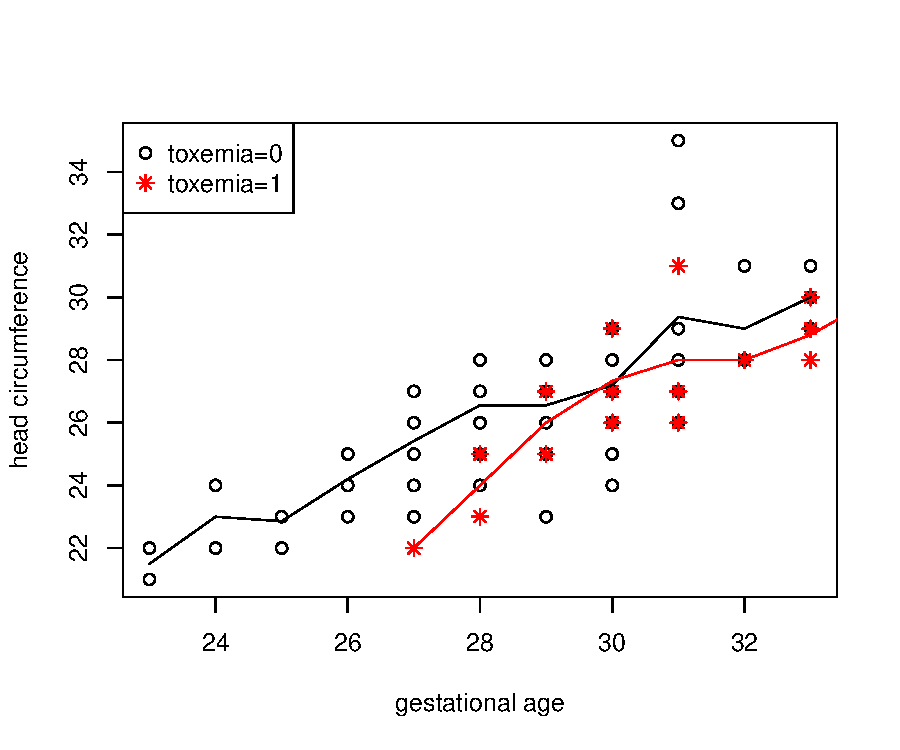
\includegraphics[width=\maxwidth]{figure/unnamed-chunk-15-1} 

}


\end{knitrout}
%\end{noindent}
\subsubsection{Equivalently: Fit a Weighted Regression}
%\begin{noindent}
\begin{knitrout}
\definecolor{shadecolor}{rgb}{0.969, 0.969, 0.969}\color{fgcolor}\begin{kframe}
\begin{alltt}
\hlkwd{library}\hlstd{(survey)}
\hlstd{design.ps} \hlkwb{<-} \hlkwd{svydesign}\hlstd{(}\hlkwc{ids} \hlstd{=} \hlopt{~}\hlnum{1}\hlstd{,} \hlkwc{weights} \hlstd{=} \hlopt{~}\hlstd{IPTW,} \hlkwc{data} \hlstd{= ds)}
\hlstd{msm1} \hlkwb{<-} \hlkwd{svyglm}\hlstd{(pcs} \hlopt{~} \hlstd{homeless,} \hlkwc{design} \hlstd{= design.ps)}
\hlkwd{summary}\hlstd{(msm1)}\hlopt{$}\hlstd{coef}
\end{alltt}
\begin{verbatim}
             Estimate Std. Error   t value      Pr(>|t|)
(Intercept) 48.623563  0.7519392 64.664225 2.971552e-230
homeless    -1.302807  1.0744770 -1.212504  2.259544e-01
\end{verbatim}
\end{kframe}
\end{knitrout}
%\end{noindent}
Note: the standard error from the survey package provides the
robust standard error and correct $p$-value.
\subsection{Double-Robust Estimation}
\begin{enumerate}[1.]
      \item Fit a logistic model for the propensity score.
            %\begin{noindent}
\begin{knitrout}
\definecolor{shadecolor}{rgb}{0.969, 0.969, 0.969}\color{fgcolor}\begin{kframe}
\begin{alltt}
\hlstd{glm1} \hlkwb{<-} \hlkwd{glm}\hlstd{(homeless} \hlopt{~} \hlstd{age} \hlopt{+} \hlkwd{factor}\hlstd{(female)} \hlopt{+} \hlstd{i1} \hlopt{+} \hlstd{mcs,} \hlkwc{family} \hlstd{= binomial)}
\hlstd{PS} \hlkwb{<-} \hlstd{glm1}\hlopt{$}\hlstd{fitted.values}
\hlkwd{summary}\hlstd{(glm1)}\hlopt{$}\hlstd{coef}
\end{alltt}
\begin{verbatim}
                    Estimate  Std. Error   z value     Pr(>|z|)
(Intercept)     -0.658258820 0.518953077 -1.268436 2.046423e-01
age              0.013659005 0.012965104  1.053521 2.921024e-01
factor(female)1 -0.454530491 0.237010899 -1.917762 5.514120e-02
i1               0.024878024 0.005781542  4.303009 1.684943e-05
mcs             -0.009983455 0.007768247 -1.285162 1.987357e-01
\end{verbatim}
\end{kframe}
\end{knitrout}
      %\end{noindent}
      \item Fit regression model for the outcome using data from the
            treatment group only, predict for all subjects.
            %\begin{noindent}
\begin{knitrout}
\definecolor{shadecolor}{rgb}{0.969, 0.969, 0.969}\color{fgcolor}\begin{kframe}
\begin{alltt}
\hlstd{out1} \hlkwb{<-} \hlkwd{lm}\hlstd{(pcs} \hlopt{~} \hlstd{age} \hlopt{+} \hlkwd{factor}\hlstd{(female)} \hlopt{+} \hlstd{i1} \hlopt{+} \hlstd{mcs,} \hlkwc{subset} \hlstd{= (homeless} \hlopt{==}
  \hlnum{1}\hlstd{))}
\hlstd{m1} \hlkwb{<-} \hlkwd{predict}\hlstd{(out1, ds)}
\hlkwd{summary}\hlstd{(out1)}\hlopt{$}\hlstd{coef}
\end{alltt}
\begin{verbatim}
                   Estimate Std. Error   t value     Pr(>|t|)
(Intercept)     55.79947502 3.44908558 16.178049 2.007994e-38
age             -0.27753512 0.08846710 -3.137156 1.958233e-03
factor(female)1 -4.01357667 1.78089142 -2.253690 2.527913e-02
i1              -0.06712578 0.03089995 -2.172359 3.098149e-02
mcs              0.11537037 0.05955119  1.937331 5.408570e-02
\end{verbatim}
\end{kframe}
\end{knitrout}
      %\end{noindent}
      \item Fit a regression model for the outcome (same form as above)
            using data from the control group only, predict for all.
            %\begin{noindent}
\begin{knitrout}
\definecolor{shadecolor}{rgb}{0.969, 0.969, 0.969}\color{fgcolor}\begin{kframe}
\begin{alltt}
\hlstd{out0} \hlkwb{<-} \hlkwd{lm}\hlstd{(pcs} \hlopt{~} \hlstd{age} \hlopt{+} \hlkwd{factor}\hlstd{(female)} \hlopt{+} \hlstd{i1} \hlopt{+} \hlstd{mcs,} \hlkwc{subset} \hlstd{= (homeless} \hlopt{==}
  \hlnum{0}\hlstd{))}
\hlstd{m0} \hlkwb{<-} \hlkwd{predict}\hlstd{(out0, ds)}
\hlkwd{summary}\hlstd{(out0)}\hlopt{$}\hlstd{coef}
\end{alltt}
\begin{verbatim}
                  Estimate Std. Error    t value     Pr(>|t|)
(Intercept)     59.6411734 3.79405564 15.7196359 1.027021e-38
age             -0.2676526 0.09564903 -2.7982780 5.556571e-03
factor(female)1 -4.1990531 1.56235123 -2.6876499 7.701442e-03
i1              -0.1034846 0.04562826 -2.2679935 2.422283e-02
mcs              0.0397022 0.05052110  0.7858537 4.327316e-01
\end{verbatim}
\end{kframe}
\end{knitrout}
      %\end{noindent}
      \item Plug in predicted values into the expression for $ \hat{\tau}_{\DR} $.
            %\begin{noindent}
\begin{knitrout}
\definecolor{shadecolor}{rgb}{0.969, 0.969, 0.969}\color{fgcolor}\begin{kframe}
\begin{alltt}
\hlstd{DR.est} \hlkwb{<-} \hlkwd{mean}\hlstd{((homeless} \hlopt{*} \hlstd{pcs} \hlopt{-} \hlstd{(homeless} \hlopt{-} \hlstd{PS)} \hlopt{*} \hlstd{m1)}\hlopt{/}\hlstd{PS)} \hlopt{-}
  \hlkwd{mean}\hlstd{(((}\hlnum{1} \hlopt{-} \hlstd{homeless)} \hlopt{*} \hlstd{pcs} \hlopt{+} \hlstd{(homeless} \hlopt{-} \hlstd{PS)} \hlopt{*} \hlstd{m0)}\hlopt{/}\hlstd{(}\hlnum{1} \hlopt{-} \hlstd{PS))}
\hlstd{DR.est}
\end{alltt}
\begin{verbatim}
[1] -1.211244
\end{verbatim}
\end{kframe}
\end{knitrout}
      %\end{noindent}
      \item Use the same bootstrap technique to obtain standard error as in
            IPW\@.
\end{enumerate}
\subsubsection{Summary}
Recall estimates of the ACE from other approaches:
\begin{itemize}
      \item Naive unadjusted: $ -2.06\;(1.013) $.
      \item Matching: $ -1.28\;(1.231) $.
      \item Stratification: $ (-1.79,0.20,-1.67,-1.99) $ [average difference $ -1.31 $].
      \item IPW\@: $ -1.30\;(1.075) $.
      \item Double-Robust: $ -1.21\;(1.02) $.
\end{itemize}
\subsubsection{Checking Balance}
How do we know if a propensity score based method did a good
job or not?
\begin{itemize}
      \item Recall $ X\indep \bigl(A\mid \ps{X}\bigr) $. If the propensity score model is correct, it should balance the
            covariates after matching/stratification/IPW.
      \item Check balance. In IPW,
            \[ w_i=\begin{dcases}
                        \frac{1}{\estps{X_i}},   & \text{if $A_i=1$}, \\
                        \frac{1}{1-\estps{X_i}}, & \text{if $A_i=0$}. \\
                  \end{dcases} \]
\end{itemize}
\begin{Regular}{Absolute Standardized Mean Difference (ASMD)}
      \[ \ASMD^{(j)}=\frac{\abs{\bar{X}_{j,1}^w-\bar{X}_{j,0}^w}}{\sd{X_{j,1}}},\; j=1,\ldots,p, \]
      \[ \ASMD\text{ mean}=\sum_{j=1}^{p}\frac{\ASMD^{(j)}}{p}, \]
      where
      \begin{itemize}
            \item $ \bar{X}_{j,1}^w=\frac{\sum w_i A_i X_{ij}}{\sum w_i A_i} $ is the weighted mean of $ X_j $ in the treatment group;
            \item $ \bar{X}_{j,0}^w=\frac{\sum w_i(1-A_i)X_{ij}}{\sum w_i(1-A_i)} $ is the weighted mean of $ X_j $ in the control group;
            \item $ \sd{X_{j,1}} $ is the unweighted standard deviation of $ X_j $ in the treatment group.
      \end{itemize}
      Instead, we can also look at
      \[ \ASMD\text{ max}=\max_j \ASMD^{(j)}\quad\text{or}\quad\ASMD\text{ mean}=\mathop{\text{median}}_j\ASMD^{(j)}.  \]
\end{Regular}
\begin{Regular}{Kolmogorov-Smirnov (KS) Statistic}
      \[ \text{KS}^{(j)}=\sup\abs*{F_{1,n_1}^w(X_{j,1})-F_{0,n_0}^w(X_{j,0})}, \]
      \[ \text{KS mean}=\sum_{j=1}^{p}\frac{\text{KS}^{(j)}}{p}, \]
      where
      \begin{itemize}
            \item $ F_{1,n_1}^w(X_{j,1}) $ is the weighted empirical cdf of $ X_j $ in the treatment group;
            \item $ F_{0,n_0}^w(X_{j,0}) $ is the weighted empirical cdf of $ X_j $ in the control group.
      \end{itemize}
\end{Regular}
%\begin{noindent}

%\end{noindent}
\begin{itemize}
      \item Usually, if $ \ASMD < 0.2 $ (or $0.1$), we say that the covariates
            are balanced across treatment groups and conclude the
            propensity score based method did a good job.
      \item The \texttt{std.diff} function posted on LEARN computes ASMD for
            each covariate. For categorical variables with $K$ levels, $K$
            indicator variables will be generated for each level, and ASMD
            values will be calculated for each level.
      \item \texttt{std.diff(u,z,w)}:
            \begin{itemize}
                  \item \texttt{u}: the covariate;
                  \item \texttt{z}: treatment indicator;
                  \item \texttt{w}: weights to be applied.
            \end{itemize}
      \item Checking balance with the IPW approach:
            %\begin{noindent}
\begin{knitrout}
\definecolor{shadecolor}{rgb}{0.969, 0.969, 0.969}\color{fgcolor}\begin{kframe}
\begin{alltt}
\hlkwd{std.diff}\hlstd{(age, homeless, IPTW)}
\end{alltt}
\begin{verbatim}
[1] 0.09585512
\end{verbatim}
\begin{alltt}
\hlkwd{std.diff}\hlstd{(}\hlkwd{factor}\hlstd{(female), homeless, IPTW)}
\end{alltt}
\begin{verbatim}
[1] 0.09554836 0.09554836
\end{verbatim}
\begin{alltt}
\hlkwd{std.diff}\hlstd{(i1, homeless, IPTW)}
\end{alltt}
\begin{verbatim}
[1] 0.2343231
\end{verbatim}
\begin{alltt}
\hlkwd{std.diff}\hlstd{(mcs, homeless, IPTW)}
\end{alltt}
\begin{verbatim}
[1] 0.07989432
\end{verbatim}
\begin{alltt}
\hlcom{# An equivalent way:}
\hlstd{x} \hlkwb{<-} \hlkwd{data.frame}\hlstd{(age,} \hlkwd{factor}\hlstd{(female), i1, mcs)}
\hlkwd{sapply}\hlstd{(x, std.diff, homeless, IPTW)}
\end{alltt}
\begin{verbatim}
$age
[1] 0.09585512

$factor.female.
[1] 0.09554836 0.09554836

$i1
[1] 0.2343231

$mcs
[1] 0.07989432
\end{verbatim}
\end{kframe}
\end{knitrout}
      %\end{noindent}
      \item Checking balance with the matching approach:
            %\begin{noindent}
\begin{knitrout}
\definecolor{shadecolor}{rgb}{0.969, 0.969, 0.969}\color{fgcolor}\begin{kframe}
\begin{alltt}
\hlstd{match} \hlkwb{<-} \hlkwd{c}\hlstd{(rr}\hlopt{$}\hlstd{index.treated, rr}\hlopt{$}\hlstd{index.control)}
\hlstd{x.matched} \hlkwb{<-} \hlstd{x[match, ]}
\hlstd{homeless.matched} \hlkwb{<-} \hlstd{homeless[match]}
\hlstd{w} \hlkwb{<-} \hlkwd{rep}\hlstd{(}\hlnum{1}\hlstd{,} \hlkwd{length}\hlstd{(match))}
\hlkwd{sapply}\hlstd{(x.matched, std.diff, homeless.matched, w)}
\end{alltt}
\begin{verbatim}
$age
[1] 0.03229325

$factor.female.
[1] 0.1205278 0.1205278

$i1
[1] 0.05847934

$mcs
[1] 0.05000506
\end{verbatim}
\end{kframe}
\end{knitrout}
      %\end{noindent}
\end{itemize}
\subsubsection{Summary}
Steps in a propensity score analysis:
\begin{enumerate}[1.]
      \item Estimate the propensity score using data $ (A_i,X_i) $, $ i=1,\ldots,n $.
      \item Select a method for propensity score adjustment:
            \begin{itemize}
                  \item Matching.
                  \item Stratification.
                  \item Inverse Probability Weighting (IPW).
                  \item Double-Robust Estimation.
            \end{itemize}
      \item Assess the balance between the treated and control groups:
            \begin{itemize}
                  \item If the covariates are balanced, go to the final step.
                  \item If the covariates are not balanced, the fitted propensity score
                        model is not good enough; refine the model.
            \end{itemize}
      \item Fit an outcome model between the treatment and the
            outcome variable using the estimated propensity scores.
\end{enumerate}

\chapter{Marginal Structural Models}
\makeheading{Week 5}{\daterange{2022-01-31}{2022-02-04}}%chktex 8
Reference: Robins, James M., Miguel Angel Hernan, and Babette
Brumback. ``Marginal structural models and causal inference in
epidemiology.'' (2000): 550-560.
\section{MSM}
\subsection*{Definition}
\begin{itemize}
      \item In regression models, we assume
            \[ \E{Y\given A=a}=\beta_0+\beta_1a. \]
            LHS represents ``average'' response in members of the population who actually received treatment $ a $.
      \item In MSMs, we assume
            \[ \E{Y^a}=\beta_0^*+\beta_1^*a. \]
            LHS represents ``average'' response under treatment $a$ in the
            entire population; MSMs model the potential outcomes
            directly.
      \item If $ A $ is unconfounded, $ \beta_1^*=\beta_1 $ because
            \[ \E{Y\given A=a}=\E{Y^a\given A=a}=\E{Y^a}. \]
      \item If $ A $ is confounded, $ \beta_1^*\ne \beta_1 $.
            \begin{itemize}
                  \item $\beta_1^*$ cannot be directly estimated.
                  \item Idea: use inverse probability weighting (IPW) to create a
                        pseudo-population in which $A$ is unconfounded.
            \end{itemize}
\end{itemize}
\subsection*{Parameters of Interest}
If both $A$ and $Y$ are binary, recall
\begin{itemize}
      \item \textbf{Crude excess risk}:
            \[ \Prob{Y=1\given A=1}-\Prob{Y=1\given A=0}. \]
      \item \textbf{Crude relative risk}:
            \[ \frac{\Prob{Y=1\given A=1}}{\Prob{Y=1\given A=0}}. \]
      \item \textbf{Crude odds ratio}:
            \[ \frac{\Prob{Y=1\given A=1}/\Prob{Y=0\given A=1}}{\Prob{Y=1\given A=0}/\Prob{Y=0\given A=0}}. \]
\end{itemize}
For comparison,
\begin{itemize}
      \item \textbf{Crude excess risk}:
            \[ \Prob{Y=1\given A=1}-\Prob{Y=1\given A=0}. \]
      \item \textbf{Causal relative risk}:
            \[ \frac{\Prob{Y^1=1}}{\Prob{Y^0=1}}. \]
      \item \textbf{Causal odds ratio}:
            \[ \frac{\Prob{Y^1=1}/\Prob{Y^1=0}}{\Prob{Y^0=1}/\Prob{Y^0=0}}. \]
\end{itemize}
Causal ER, RR and OR can be expressed in terms of parameters of
the following MSMs:
\begin{itemize}
      \item $ \Prob{Y^a=1}=\psi_0+\psi_1 a\implies\text{Causal ER}=\psi_1 $.
      \item $ \log[\big]{\Prob{Y^a=1}}=\theta_0+\beta_1a\implies\text{Causal RR}=e^{\theta_1} $.
      \item $ \logit[\big]{\Prob{Y^a=1}}=\beta_0+\beta_1a\implies\text{Causal OR}=e^{\beta_1} $.
\end{itemize}
\subsection*{Causal Diagram}
TODO
\subsection*{Inverse Probability Weighting}
The causal quantities can be consistently estimated in (b)--(c) by
fitting the corresponding regression model ($Y \sim A$) with IPW
weights:
\[ w_i=\frac{1}{\Prob{A=A_i\given X=X_i}}. \]
\[ \hat{w}_i=\begin{dcases}
            \frac{1}{\estps{X_i}},   & A_i=1, \\
            \frac{1}{1-\estps{X_i}}, & A_i=0.
      \end{dcases} \]
To avoid extreme weights, we may use stabilized weights:
\[ sw_i=\frac{\Prob{A=A_i}}{\Prob{A=A_i\given X=X_i}}. \]
\begin{itemize}
      \item If we have a binary treatment and a binary outcome with a
            single time point, unstabilized and stabilized weights yield the
            same estimates;
      \item Otherwise, stabilized weights yield more efficient estimates.
\end{itemize}
\section{Example 1: Why does IPW work?}
\[ \begin{array}{ccccc}
            \toprule
                         & \multicolumn{2}{c}{X=1} & \multicolumn{2}{c}{X=0}             \\
                         & A=1                     & A=0                     & A=1 & A=0 \\
            Y=1          & 108                     & 24                      & 20  & 40  \\
            Y=0          & 252                     & 16                      & 30  & 10  \\
            \text{Total} & 360                     & 40                      & 50  & 50  \\
            \bottomrule
      \end{array} \]
\begin{itemize}
      \item $ \Prob{A=1\given X=1}=0.9 $ and $ \Prob{A=1\given X=0}=0.5 $ both imply
            $ X $ and $ A $ are confounded.
\end{itemize}
Aggregated Data:
\[ \begin{array}{lcc}
            \toprule
                         & A=1 & A=0 \\
            Y=1          & 128 & 64  \\
            Y=0          & 282 & 26  \\
            \text{Total} & 410 & 90  \\
            \bottomrule
      \end{array} \]
\begin{itemize}
      \item Crude relative risk $ =\Prob{Y=1\given A=1}/\Prob{Y=1\given A=0}=\frac{128/410}{64/90}=0.44 $.
\end{itemize}
We can calculate causal relative risk by conditioning on $X$
(assuming the ignorability assumption holds):
\begin{align*}
      \Prob{Y^1=1}
       & =\Prob{Y=1\given A=1,X=1}\Prob{X=1}+\Prob{Y=1\given A=1,X=0}\Prob{X=0} \\
       & =\frac{108}{360}\frac{4}{5}+\frac{20}{50}\frac{1}{5}                   \\
       & =0.32.
\end{align*}
Similarly,
\begin{align*}
      \Prob{Y^0=1}
       & =\Prob{Y=1\given A=0,X=1}\Prob{X=1}+\Prob{Y=1\given A=0,X=0}\Prob{X=0} \\
       & =\frac{24}{40}\frac{4}{5}+\frac{40}{50}\frac{1}{5}                     \\
       & =0.64.
\end{align*}
Therefore, Causal Relative Risk $=\Prob{Y^1=1}/\Prob{Y^0=1}=0.32/0.64=0.5$.

Another approach is performing Inverse Probability Weighting:
\[ \begin{array}{ccccccc}
            \toprule
            X & A & Y & n~\text{(observed)} & \Prob{A\given X} & w    & N~\text{(pseudo)} \\
            1 & 1 & 1 & 108                 & 0.9              & 1.11 & 120               \\
            1 & 1 & 0 & 252                 & 0.9              & 1.11 & 280               \\
            1 & 0 & 1 & 24                  & 0.1              & 10   & 240               \\
            1 & 0 & 0 & 16                  & 0.1              & 10   & 160               \\
            0 & 1 & 1 & 20                  & 0.5              & 2    & 40                \\
            0 & 1 & 0 & 30                  & 0.5              & 2    & 60                \\
            0 & 0 & 1 & 40                  & 0.5              & 2    & 80                \\
            0 & 0 & 0 & 10                  & 0.5              & 2    & 20                \\
            \bottomrule
      \end{array} \]
Pseudopopulation Created by IPW with Binary $A$ Stratified by the
Confounder $X$:
\[ \begin{array}{ccccc}
            \toprule
                         & \multicolumn{2}{c}{X=1} & \multicolumn{2}{c}{X=0}             \\
                         & A=1                     & A=0                     & A=1 & A=0 \\
            Y=1          & 120                     & 240                     & 40  & 80  \\
            Y=0          & 280                     & 160                     & 60  & 20  \\
            \text{Total} & 400                     & 400                     & 100 & 100 \\
            \bottomrule
      \end{array} \]
\begin{itemize}
      \item $ \Prob{A=1\given X=1}= \Prob{A=1\given X=0}=0.5 $ imply $ X $ and $ A $ are confounded.
\end{itemize}
Aggregated Data from the Pseudopopulation:
\[ \begin{array}{lcc}
            \toprule
                         & A=1 & A=0 \\
            Y=1          & 160 & 320 \\
            Y=0          & 340 & 180 \\
            \text{Total} & 500 & 500 \\
            \bottomrule
      \end{array} \]
\begin{itemize}
      \item Crude relative risk $ =\Prob{Y=1\given A=1}/\Prob{Y=1\given A=0}=\frac{160/500}{320/500}=0.5 $.
\end{itemize}
\section{Example 2: Fit MSM for Continuous Treatments}
Early Dieting in Girls Study: a longitudinal study that aims to examine
parental influences on daughters' growth and development from ages 5--15.
\begin{itemize}
      \item Reference: Zhu, Y., Coffman, D. L., Ghosh, D. (2015). A boosting algorithm for estimating generalized propensity
            scores with continuous treatments. Journal of causal inference, 3(1), 25-40.
\end{itemize}
\begin{itemize}
      \item Treatment (M2WTCON):
            \begin{itemize}
                  \item mother's overall weight concern, calculated as the average
                        score of five likert-scale (1-5) questions
                  \item measured at girls' age 7
                  \item which can be regarded as a continuous treatment variable
            \end{itemize}
      \item Outcome (earlydiet): whether the daughter diets between
            ages 7 and 11, which is binary.
      \item Baseline confounders (50 covariates in total):
            \begin{itemize}
                  \item family history of diabetes and obesity, family income, etc
                  \item daughter's disinhibition, daughter's body esteem, etc
                  \item mother's perception of mother's current size and mother's
                        satisfaction with daughter's current body, etc.
            \end{itemize}
\end{itemize}
The following is one sample question in the weight concern
questionnaire:
\begin{enumerate}
      \item How afraid are you of gaining 3 pounds:
            \begin{enumerate}[(1)]
                  \item Not afraid
                  \item Slightly afraid
                  \item Moderately afraid
                  \item Very afraid
                  \item Terrified
            \end{enumerate}
\end{enumerate}
\begin{itemize}
      \item Fit a marginal structural model
            \[ \logit[\big]{\Prob{Y^a=1}}=\beta_0^*+\beta_1^*a, \]
            where $ a\in[a_1,a_2] $ and $ \beta_1^* $ is the causal log odds ratio for $1$
            unit increase in the treatment (dosage) $A$.
      \item The causal effect $ \beta_1^* $ can be consistently estimated by fitting
            the corresponding regression model
            \[ \logit[\big]{\Prob{Y=1}}=\beta_0+\beta_1a, \]
            using IPW where
            \[ sw_i=\frac{f(A_i)}{f(A_i\mid X_i)},\; i=1,\ldots,n, \]
            where $f(\:\cdot\:)$is the unconditional density and  $f(\:\cdot\:\mid\:\cdot\:)$ is the
            conditional density.
      \item Problem: when $X$ is of even moderate dimension, estimate the
            conditional density is challenging.
      \item Solution: use normal approximation to estimate the
            unconditional and conditional density.
      \item Using normal density, we can estimate $f (A_i )$ by:
            \[ \hat{f}(A_i)=\frac{1}{\sqrt{2\pi}\hat{\sigma}}\exp*{-\frac{(A_i-\hat{\mu})^2}{2\hat{\sigma}^2}}, \]
            where $ \hat{\mu} $ and $ \hat{\sigma} $ are the sample mean and SD of $ A_1,\ldots,A_n $.
      \item Assume
            \[ A_i=X_i^\top \beta+\varepsilon_i, \]
            where $ \varepsilon_i \sim \N{0,\sigma^2} $.
      \item Let $ r_i=A_i-X_i^\top \hat{\beta} $, we can approximate $ f(A_i\mid X_i) $ by $ \hat{f}(r_i\mid X_i) $:
            \[ \hat{f}(A_i\mid X_i)=\hat{f}(r_i\mid X_i)=\frac{1}{\sqrt{2\pi}\tilde{\sigma}}\exp*{-\frac{(A_i-X_i\hat{\beta})^2}{2\tilde{\sigma}^2}}, \]
            where $ \tilde{\sigma}^2 $ is the mean-squared error (MSE).
\end{itemize}
R Code, not public.
\end{document}
